\documentclass[conference]{IEEEtran}
\IEEEoverridecommandlockouts
\usepackage{cite}
\usepackage{amsmath,amssymb,amsfonts}
\usepackage{graphicx}
\usepackage{booktabs}
\usepackage{xcolor}
\usepackage{url}
\usepackage[hidelinks]{hyperref}
\usepackage{textcomp}

% This TeX install lacks Helvetica (phv) and Courier (pcr) metrics; keep Times
% for body text and fall back to Computer Modern for sans/mono so it compiles.
\renewcommand{\sfdefault}{cmss}
\renewcommand{\ttdefault}{cmtt}

% Float placement: keep figures on/near the page that references them rather
% than letting many [t]-only floats queue up and drift pages later.
\renewcommand{\topfraction}{0.92}
\renewcommand{\bottomfraction}{0.85}
\renewcommand{\textfraction}{0.08}
\renewcommand{\floatpagefraction}{0.75}
\renewcommand{\dbltopfraction}{0.92}
\renewcommand{\dblfloatpagefraction}{0.75}
\setcounter{topnumber}{3}
\setcounter{bottomnumber}{2}
\setcounter{totalnumber}{4}
\setcounter{dbltopnumber}{2}

\begin{document}

\title{Sensorless Position and Force Estimation for a\\
Double-Acting Hydraulic Cylinder Using Pressure\\
and Flow Signals}

\author{\IEEEauthorblockN{Jyotirmoy Ray}
\IEEEauthorblockA{Wipro Research\\
\texttt{jyotirmoy.ray@wiproresearch.in}}}

\maketitle

\begin{abstract}
A double-acting hydraulic cylinder couples oil pressure and flow to piston
position and force. We ask whether, using only pressure and flow transducers and
no position sensor, position can be held within $\pm 5$\,cm and net force within
$\pm 12\,\%$ of full scale across the full stroke and a $0$--$50\,$\textdegree C
temperature range, under realistic sensor noise and bias. We answer with an
offline study in which the cylinder, valve, supply, end-stops and controller are
modelled in Hopsan, a transmission-line fluid-power simulator that supplies
synthetic---and then deliberately corrupted---sensor streams to a complementary
observer: position from flow-continuity velocity, re-zeroed at the end-stops, and
force from the measured pressures. Across a 48-run Monte-Carlo sweep with per-run
parameter mismatch, the worst-case position error is $2.58$\,cm and the
operational force error $5.08\,\%$ FS, both within target. Ablations identify the
end-stop \emph{homing reset} as the load-bearing mechanism; sweeps over supply
pressure, bore and hose length, a head-to-head against an extended Kalman filter,
and a cross-check against a published physical experiment delimit where the scheme
holds. The result is a feasibility statement for this class of actuator and a
reusable plant-in-the-loop harness, not a hardware claim.
\end{abstract}

\begin{IEEEkeywords}
hydraulic cylinder, sensorless estimation, state observer, Hopsan, transmission
line modelling, fluid power, force estimation.
\end{IEEEkeywords}

\section{Introduction}
Hydraulic cylinders convert fluid power into linear force and motion and are the
workhorse of heavy machinery. A double-acting cylinder is a coupled system: the
oil flow rate into each chamber sets the piston velocity (and hence, by
integration, position), while the pressure difference across the piston sets the
net force. Knowing position and force is essential for closed-loop motion and for
condition monitoring, but external position sensors (LVDTs, magnetostrictive
rods, draw-wire encoders) add cost, cabling and failure modes, and are awkward to
retrofit. Pressure transducers and in-line flow meters, by contrast, are cheap,
robust and often already present for protection and diagnostics. This motivates
\emph{sensorless} estimation: recover position and force from pressure and flow
alone.

The difficulty is that the two informative channels degrade differently.
Integrating flow to get position is exact in principle but accumulates any
flow-meter \emph{bias} without bound, so a $0.5\,\%$ offset becomes metres of
drift over a duty cycle. Pressure maps to force almost directly, so force is
limited only by transducer noise. Temperature complicates both: over
$0$--$50\,$\textdegree C the oil bulk modulus (its stiffness against compression,
which sets how fast pressure builds for a given trapped-volume change), viscosity
and leakage change substantially, shifting the compressibility and leakage
corrections the estimator must make.

This paper is a deliberately scoped \emph{spike}: a time-boxed feasibility study
of one concrete actuator and duty cycle, with the explicit acceptance targets of
$\pm 5$\,cm position and $\pm 12\,\%$ full-scale (FS) force across the stroke and
the temperature range. We do not claim a new estimator class. The contributions
are: (i) a physically faithful, reproducible plant-in-the-loop harness that uses
Hopsan as the truth model, so the synthetic sensor data comes from a validated
TLM fluid-power solver rather than a bespoke script; (ii)
a complementary observer (a deliberately simple estimator that \emph{blends} two
imperfect information sources---here a fast flow-derived velocity and a slow
position correction at the end-stops---rather than running a full statistical
filter) whose drift is bounded by end-stop homing, with steady-gated bias
calibration as a refinement; and (iii) a Monte-Carlo characterisation (many runs
with randomised noise and plant parameters) across temperature, sensor-noise and
parameter-mismatch seeds showing the targets are met with margin, together with an
identification of which mechanism actually binds.

\emph{The idea in one paragraph} (Fig.~\ref{fig:principle}). The piston's speed
equals the net volumetric flow into a chamber divided by the piston area;
integrate that speed and you have position. The net force on the piston is just
the two chamber pressures times their areas. So in principle two flow meters and two pressure sensors are enough
to recover both quantities with no position sensor at all. The catch is drift: any
tiny constant error in a flow meter, once integrated, grows without bound, so the
position estimate slowly walks away from truth. The whole design is therefore
about \emph{pinning} that drift---which is what the hydraulic end-stops, where the
piston momentarily stops and its position is known exactly, let us do for free.

\emph{Roadmap.} Section~\ref{sec:plant} builds the plant model (and explains why a
transmission-line simulator suits the stiff hydraulics); Section~\ref{sec:sensors}
adds realistic sensor imperfections; Section~\ref{sec:observer} derives the
estimator from the chamber equations; Section~\ref{sec:results} reports the
Monte-Carlo sweep and then dissects \emph{which} mechanism carries the result,
tests robustness across supply pressure, cylinder size and hose length, compares
against a full Kalman filter, and validates against a published physical
experiment.

\section{Background and Related Work}
Two equations describe a hydraulic cylinder, and both come straight from
first principles. The first is conservation of volume in each chamber: oil pumped
in must either move the piston or compress the trapped fluid, so the rate of
pressure rise is the net inflow (minus the flow ``used up'' moving the piston)
divided by the chamber's compliance---this is the \emph{continuity equation}, and
the fluid bulk modulus is what converts a compressed volume into a pressure. The
second is Newton's law for the piston: mass times acceleration equals the
pressure-times-area force from each side minus friction and load. Classical
hydraulic modelling \cite{merritt1967,jelali2003hydraulic} and the servo-control
literature \cite{bobrow1998adaptive,alleyne2000force} build on exactly this pair.
Reading force from the chamber pressures is standard \cite{alleyne2000force};
sensorless \emph{position} is the harder half, because of the integration-drift
problem noted above.

\begin{figure*}[!t]
\centering
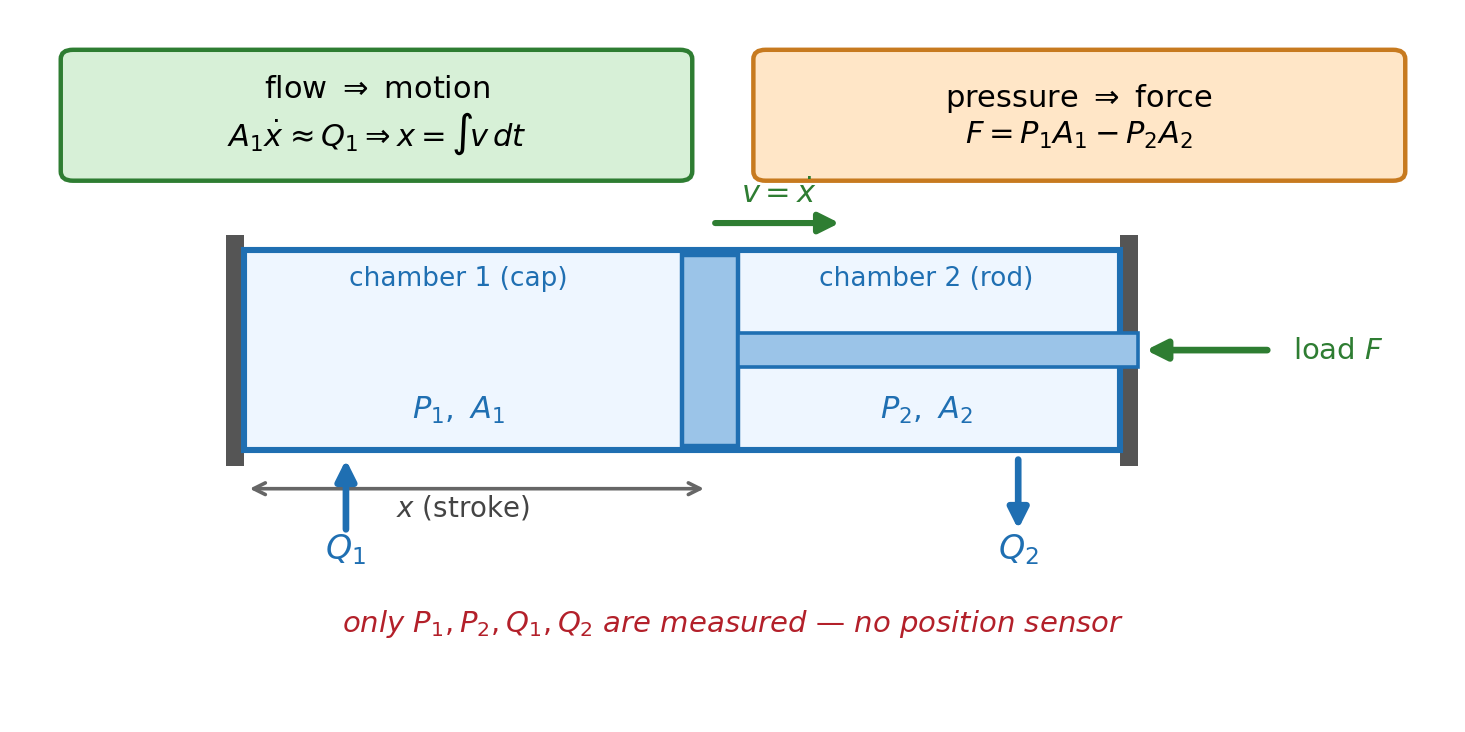
\includegraphics[width=0.84\textwidth]{../figures/fig_principle.png}
\caption{The double-acting cylinder as a coupled system, from first principles.
Oil flow into a chamber must move the piston (a flow $Q_1$ sweeps volume $A_1$ at
speed $\dot x$), so integrating the flow-derived velocity gives position; the net
force is the pressure-area difference $P_1A_1-P_2A_2$. Only the four chamber
signals $P_1,P_2,Q_1,Q_2$ are instrumented---there is no position sensor, which is
the whole point of the study.}
\label{fig:principle}
\end{figure*}
Closest to this work, Zhou et al.\ \cite{zhou2022pressure} estimate the position
of a mining-support cylinder from pressure-derived flow on a physical $400$\,L/min
rig and report errors within $5\,\%$ above $10$\,MPa; we validate against their
measurements in Sec.~\ref{sec:zhou}.

Our truth model is built in Hopsan, an open-source multi-domain simulator from
Link\"oping University \cite{axin2010hopsan,hopsanrepo}. Hopsan uses the
transmission-line method (TLM) \cite{krus1988tlm}: components communicate through
bilateral delay lines with a one-time-step transport delay, which decouples the
numerical solution of connected sub-models and gives unconditionally stable,
distributed integration. This is attractive for a plant-in-the-loop study because
the hydraulic stiffness (large $\beta$, small chamber volumes) that makes naive
explicit integration fragile is handled natively by the solver.

\section{Plant Model in Hopsan}\label{sec:plant}
The plant is the Hopsan model of Fig.~\ref{fig:model}, adapted from the
Apache-licensed ``Position Servo'' example. The double-acting cylinder
(\texttt{HydraulicCylinderC}) is connected through a 4/3 proportional servo valve
(\texttt{Hydraulic43Valve}) to a pressure-relief-limited supply; a translational
mass with hard end-stops carries the load, and a PI controller closes a position
loop around a reference source. All components are standard library parts.

Crucially for realism, the pressure and flow transducers are not at the cylinder
but at the \emph{valve manifold}, with a hose run carrying oil to the cylinder---
the usual layout on real machines, where instrumenting the moving cylinder is
exactly what one is trying to avoid. We model each hose as a Hydraulic Volume
(line compliance) followed by a laminar orifice (friction loss), giving the
TLM-legal chain valve\,$\rightarrow$\,line\,$\rightarrow$\,cylinder; the orifice
coefficient follows Hagen--Poiseuille ($\propto d^4/(\mu L)$, hence temperature
dependent) and the volume is the hose bore volume. The sensors therefore read the
manifold side, upstream of the line loss, so the estimator never sees the true
cylinder pressure exactly (Fig.~\ref{fig:manifold}; the full ISO schematic with
the hoses highlighted is Fig.~\ref{fig:canvas})---a deliberate, quantifiable
error source studied in Sec.~\ref{sec:hose}.

\begin{figure}[!tb]
\centering
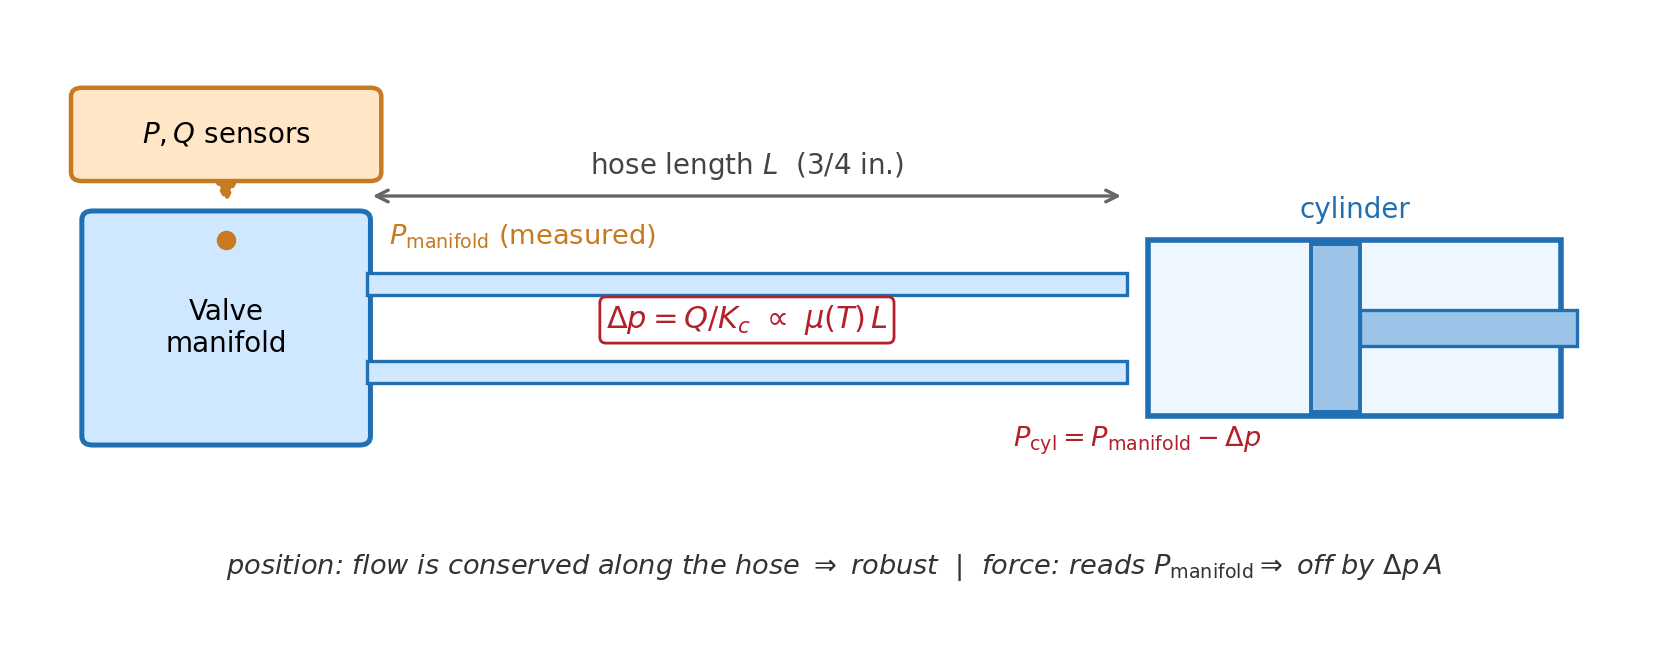
\includegraphics[width=\linewidth]{../figures/fig_manifold.png}
\caption{Manifold-located sensing. The transducers tap the valve block; a hose of
length $L$ carries oil to the cylinder, dropping pressure by $\Delta p$. Position
is unaffected (flow is conserved along the hose) but the force read-out inherits
the full $\Delta p\,A$ offset, which grows with length and with colder, more
viscous oil.}
\label{fig:manifold}
\end{figure}

\begin{figure}[!tb]
\centering
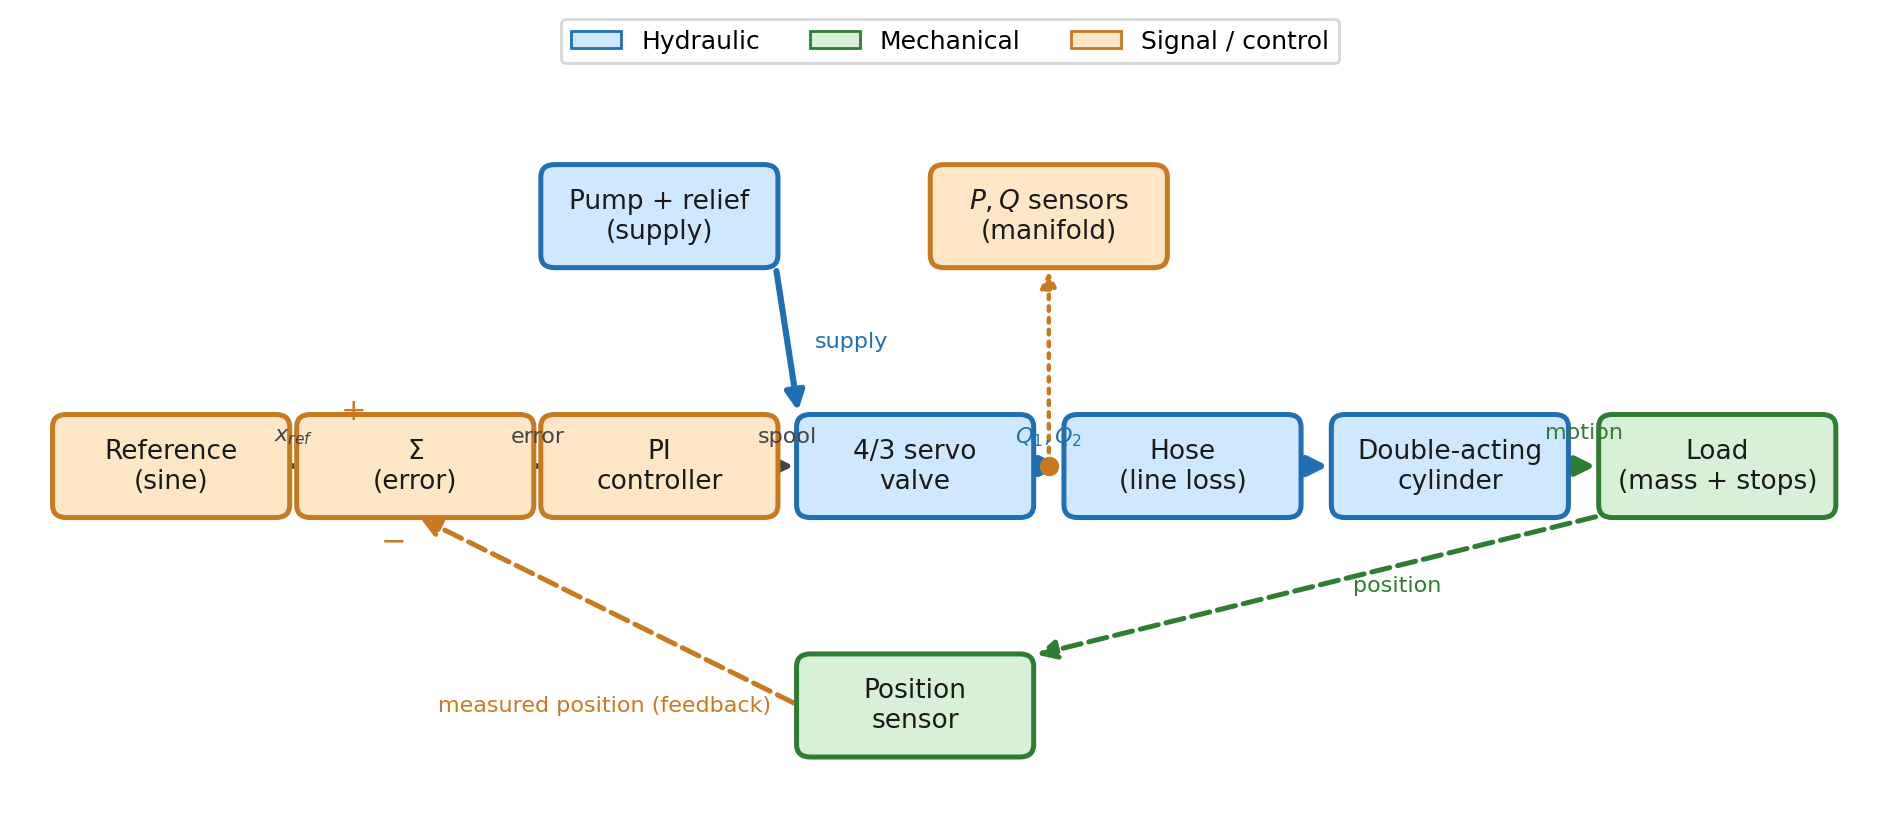
\includegraphics[width=\linewidth]{../figures/fig_hopsan_model.png}
\caption{Block schematic of the Hopsan plant: a PI position controller drives a
4/3 servo valve feeding a double-acting cylinder against a mass / end-stop load,
a relief-limited pump supplies pressure, and a position sensor closes the loop.
Blue is the hydraulic domain, green mechanical, orange signal/control. The
detailed model as built in Hopsan is shown in Fig.~\ref{fig:gui}.}
\label{fig:model}
\end{figure}

\subsection{Why a transmission-line plant: TLM versus acausal solvers}
\label{sec:tlm}
Because the entire premise of this study is that the \emph{plant}, not the
estimator, supplies ground truth, the choice of plant solver matters and is worth
making explicit. The two mainstream options for fluid power are acausal,
equation-based environments (Simscape Fluids, Modelica/Dymola, AMESim) and the
transmission-line method (TLM) used by Hopsan. They differ in how a connected
network is solved.

\textbf{Acausal solvers} treat the whole circuit as one differential-algebraic
equation (DAE) system: each component contributes constitutive equations in terms
of port efforts (pressure) and flows, and at every time step a global solver
assembles and solves the coupled system implicitly, resolving the algebraic loops
that connection imposes \cite{cellier2006continuous}. Fidelity and convenience are
high, but a hydraulic circuit is numerically \emph{stiff}: a large bulk modulus
$\beta$ acting on a small chamber volume $V$ gives a pressure mode with natural
frequency $\sim\!\sqrt{\beta A^2/(mV)}$ of many kHz, far above the mechanical
motion of interest. Resolving it forces a stiff implicit integrator (e.g.
\texttt{ode23t}/\texttt{ode15s}) with a global Newton solve per step, and stiff
events---valve transitions, end-stop contact, cavitation---can stall the step-size
controller.

\textbf{TLM} instead decouples the network physically. A fluid line has a real
propagation delay; TLM models each connection as a bilateral delay line that
carries pressure/flow ``characteristics'' with a one-time-step transport lag
\cite{johns1971tlm,krus1988tlm,axin2010hopsan}. Because a component at time $t$
sees its neighbours only through their state one step \emph{earlier}, every
component integrates locally and independently---there is no global system to
assemble, no algebraic loop to resolve, and the coupling can never inject the
spurious high-frequency feedback that destabilizes an explicit global scheme. The
characteristic impedance of each delay line provides physically-motivated
numerical damping, so the scheme is robust precisely at the stiff pressure node
that troubles a monolithic solver. The practical consequences for a plant-in-the-
loop Monte-Carlo study like ours are: (i) \emph{stability}---the stiff $\beta$/$V$
dynamics are handled natively rather than by shrinking a global step; (ii)
\emph{speed and scale}---local, decoupled updates parallelize across components and
cores, so the dozens of multi-second runs behind every sweep here are cheap; and
(iii) \emph{determinism}---a fixed transport delay means fixed compute per step,
which is also why TLM is favoured for hardware-in-the-loop.

Two honest caveats keep this in proportion. First, TLM's signature advantage, the
faithful capture of pressure-wave propagation, is decisive for \emph{long
transmission lines} but marginal for a single lumped actuator, whose chamber
delays are microseconds; here the win is numerical (stability, speed), not
wave-fidelity. Second, a numerically robust \emph{plant} does not make the
\emph{estimation} problem easy: the stiff velocity--pressure oscillator still has
to be confronted in the observer and EKF (Sec.~\ref{sec:ekf}), independent of how
the truth was generated. We use Hopsan because it gives a fast, stable, free,
FMI-exportable truth model for the stiff regime we sweep; the estimator results
that follow are agnostic to that choice.

\subsection{Governing equations}
For the cap-side (chamber 1, area $A_1$) and rod-side (chamber 2, area $A_2$)
chambers, Hopsan's cylinder enforces the continuity relation
\begin{equation}
\dot{P}_i = \frac{\beta_e}{V_i(x)}\Big(Q_i - (\pm)A_i \dot{x} - q_{\text{leak}}\Big),
\label{eq:cont}
\end{equation}
with position-dependent volumes $V_1(x)=V_{01}+A_1 x$ and
$V_2(x)=V_{02}+A_2(s_\ell-x)$, laminar cross-piston leakage
$q_{\text{leak}}=C_{\text{leak}}(P_1-P_2)$, and effective bulk modulus $\beta_e$.
The piston obeys
\begin{equation}
m\ddot{x} = P_1 A_1 - P_2 A_2 - F_{\text{fric}}(\dot{x}) - F_{\text{load}}
            + F_{\text{stop}}(x,\dot{x}),
\label{eq:newton}
\end{equation}
where $F_{\text{fric}}$ combines viscous, Coulomb and stiction (static $>$
kinetic) terms, and the valve passes a turbulent-orifice flow
$Q = C_q\,w\,x_v\sqrt{2\,\Delta P/\rho}$ set by a second-order spool of finite
bandwidth. Equations~\eqref{eq:cont}--\eqref{eq:newton} are solved by Hopsan
with the TLM scheme; we do not integrate them ourselves.

\subsection{Temperature parameterization}
Hopsan exposes $\beta_e$, $C_{\text{leak}}$ and the viscous-friction coefficient
as \emph{constant} parameters; it has no built-in temperature dependence. We
therefore cover the $0$--$50\,$\textdegree C envelope by re-parameterising the
model once per run from the curves of Fig.~\ref{fig:fluid}: a bulk modulus that
stiffens when cold, a Vogel-like viscosity that rises sharply when cold, and a
leakage coefficient that scales with $1/\mu(T)$ (more leakage when hot and thin).
Each Monte-Carlo run is at one steady oil temperature, so constant-per-run
parameters are faithful.

\subsection{Plant realism and model mismatch}\label{sec:realism}
To avoid the trap of an estimator that secretly knows the plant, the plant
includes effects the observer does not model and is perturbed away from the
observer's nominal parameters each run:
\begin{itemize}
\item \textbf{Friction}: Coulomb + stiction (static $1.5\times$ kinetic) on the
piston, on top of viscous damping, producing stick--slip near reversals.
\item \textbf{Valve dynamics}: a finite-bandwidth second-order spool rather than
an algebraic valve.
\item \textbf{Parameter mismatch}: per run the plant's bulk modulus, cross-piston
leakage, viscous friction, dead volumes and areas are scaled by independent
log-normal factors with one-sigma spreads of $10$, $20$, $20$, $12$ and
$0.5\,\%$ respectively (representative of oil aeration/wear, seal-leakage and
hose-volume uncertainty, and machined-geometry tolerance), while the observer
keeps nominal values. This converts the sweep from a noise-robustness test into a
genuine \emph{model-mismatch} test.
\end{itemize}

\begin{figure}[!tb]
\centering
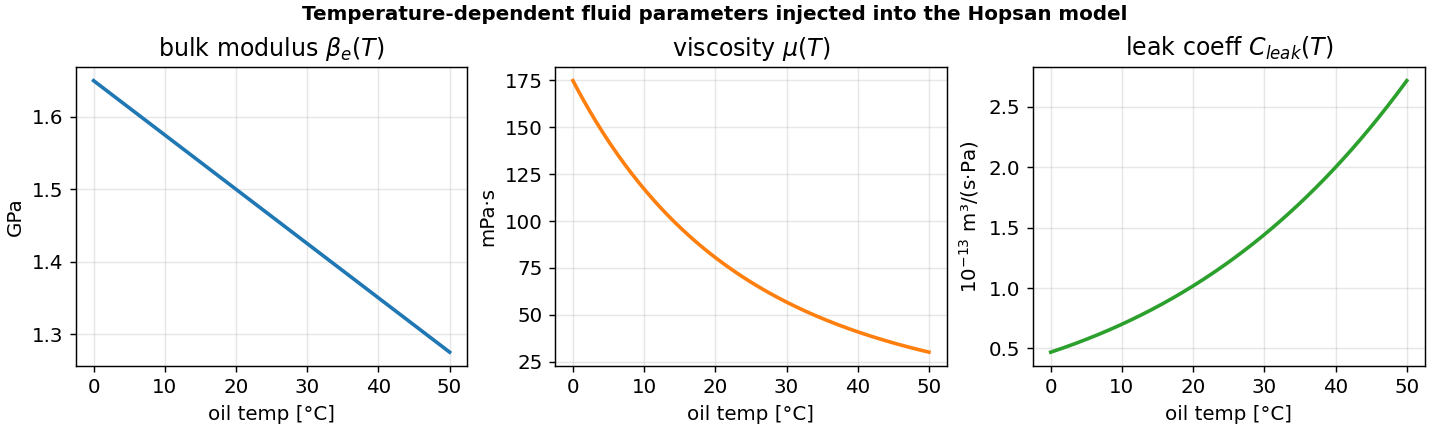
\includegraphics[width=\linewidth]{../figures/fig_fluid_temp.png}
\caption{Temperature-dependent fluid parameters injected into the Hopsan model
per run. Hopsan itself holds these constant, so the envelope is swept by
re-parameterisation.}
\label{fig:fluid}
\end{figure}

\subsection{Excitation and simulation}
Each run is simulated in Hopsan with per-run parameters (geometry, the
temperature-dependent fluid values, controller gains and the reference); the
exported pressure, flow and position time series form the truth log. The
reference is a sine of amplitude $1.1\times$ stroke, so the servo sweeps the full
stroke and seats both end-stops each half cycle; the seating events are what the
observer uses for calibration.

\begin{figure}[!tb]
\centering
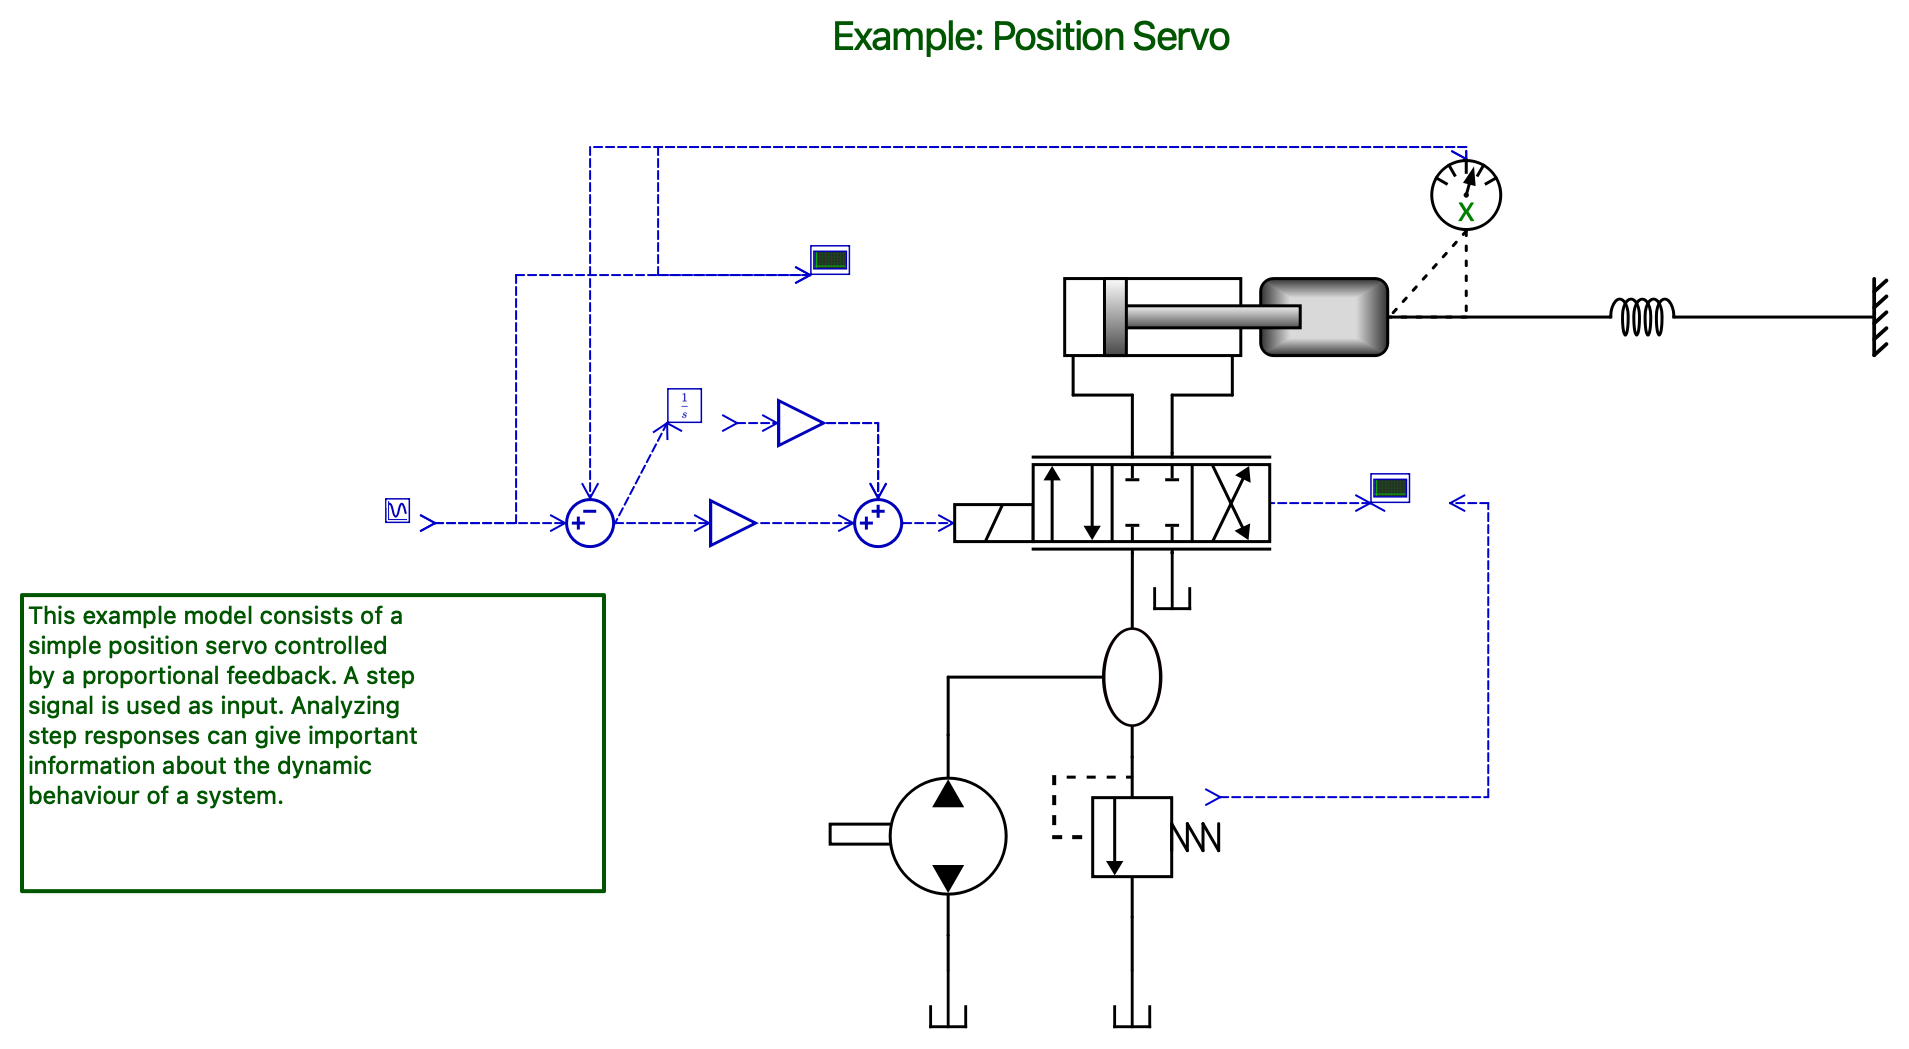
\includegraphics[width=\linewidth]{../figures/fig_hopsan_gui.png}
\caption{The Hopsan plant model with the standard ISO fluid-power symbols: the
double-acting cylinder driving a mass--spring load with the position sensor, the
4/3 servo valve, the pump and relief valve, and the blue signal/control chain
(sine reference, summation, gains, integrator, scopes). This is the model that
produces all synthetic sensor data; the block schematic of Fig.~\ref{fig:model}
is rendered independently from the \texttt{.hmf} for labelling.}
\label{fig:gui}
\end{figure}

\begin{figure*}[!t]
\centering
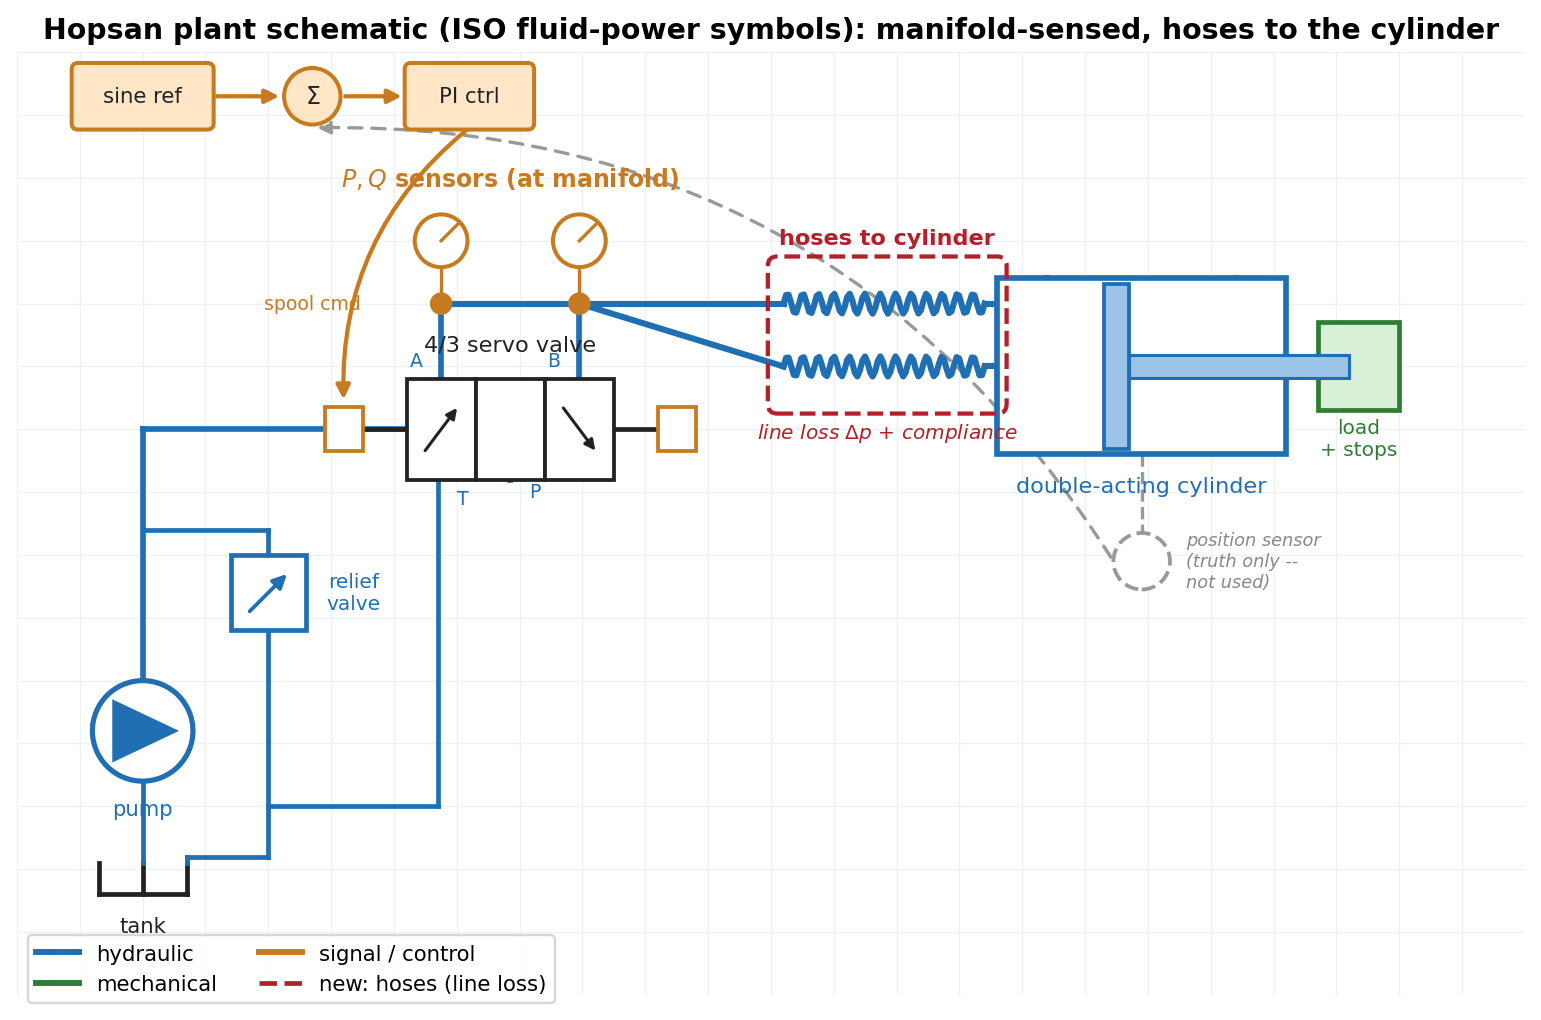
\includegraphics[width=0.95\textwidth]{../figures/fig_hopsan_canvas.png}
\caption{Annotated ISO-1219 schematic of the same plant, with the
manifold-to-cylinder hoses added this revision highlighted (red). Oil runs
tank\,$\rightarrow$\,pump\,$\rightarrow$\,relief-limited supply\,$\rightarrow$\,4/3
servo valve; the $P,Q$ transducers tap the valve manifold (ports A/B), and
\emph{flexible hoses} carry oil to the double-acting cylinder, so the sensors sit
upstream of the line drop $\Delta p$. The cylinder's own position sensor (grey) is
ground truth only and is never used by the estimator.}
\label{fig:canvas}
\end{figure*}

\section{Synthetic Sensors}\label{sec:sensors}
The clean Hopsan signals are corrupted by a transducer model that mimics
industrial-grade hardware (Table~\ref{tab:sensors}). Each channel applies, in
order: a first-order bandwidth (pressure $500$\,Hz, flow $80$\,Hz), white noise,
a per-run constant bias plus a slow bias random-walk (zero drift), a transport
delay ($1.5$\,ms), and 12-bit quantization; flow additionally gets a K-factor
nonlinearity and full-scale saturation. The flow \emph{bias} ($0.5\,\%$ FS) is
the term that defeats naive integration. Oil temperature is available only as a
noisy reading ($\pm 1\,$\textdegree C). No position or velocity is measured.
Fig.~\ref{fig:signals} shows a representative pressure/flow record: pressures
saturate near the relief setting when the piston seats, and flows reverse with
stroke direction; the faint traces are the noisy measurements the observer
actually sees.

\begin{figure}[!tb]
\centering
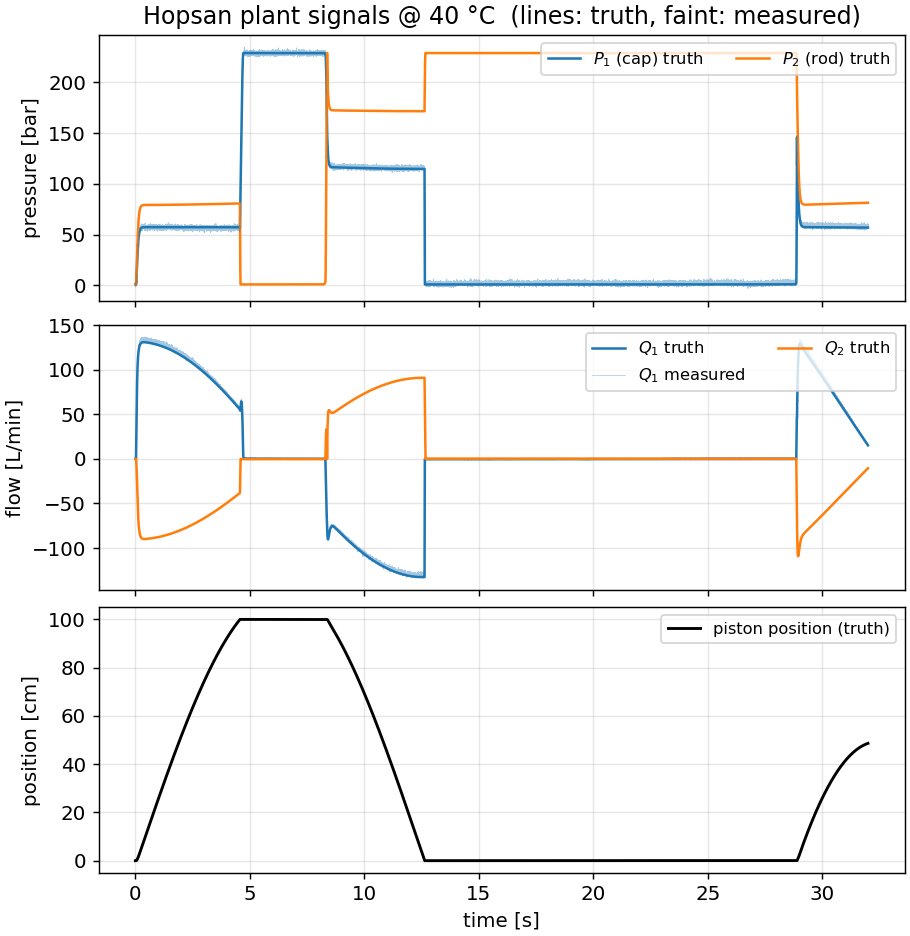
\includegraphics[width=\linewidth]{../figures/fig_signals.png}
\caption{Synthetic sensor streams from the Hopsan plant at $40\,$\textdegree C.
Chamber pressures (top) climb to the relief limit at the stops; chamber flows
(middle) reverse with direction; piston position (bottom) sweeps the full stroke.
Faint overlays are the noisy measurements.}
\label{fig:signals}
\end{figure}

\begin{table}[t]
\caption{Cylinder and sensor parameters}
\label{tab:sensors}
\centering
\small
\begin{tabular}{@{}lll@{}}
\toprule
Quantity & Value & Note\\
\midrule
Bore / rod / stroke & $100/56/1000$\,mm & \\
Moving mass & $200$\,kg & \\
Supply pressure & $210$\,bar & relief-set\\
Force full scale & $164.9$\,kN & $A_1\,P_s$\\
Pressure noise & $0.5\,\%$ FS & FS $=250$\,bar\\
Pressure bias & $0.25\,\%$ FS & per run\\
Flow noise & $1\,\%$ rdg $+0.2\,\%$ FS & FS $=160$\,L/min\\
Flow bias & $0.5\,\%$ FS & per run\\
Sensor bandwidth & $500$ / $80$\,Hz & pressure / flow\\
Transport delay & $1.5$\,ms & all channels\\
Zero drift & $0.15\,\%$ FS/s & random walk\\
Temperature sensor & $\pm 1\,$\textdegree C & noise\\
Sampling rate & $1$\,kHz & \\
\bottomrule
\end{tabular}
\end{table}

\section{Sensorless Observer}\label{sec:observer}
Position is reconstructed from the channel that actually carries it: flow. Each
chamber's continuity equation~\eqref{eq:cont}, rearranged, gives an estimate of
piston velocity from the measured flow, corrected for bias $b_i$, leakage and the
compressibility term:
\begin{align}
A_1 v_1 &= (Q_1 - b_1) - (V_1/\beta_e)\dot{P}_1 - q_{\text{leak}},\\
A_2 v_2 &= (V_2/\beta_e)\dot{P}_2 - (Q_2 - b_2) - q_{\text{leak}}.
\end{align}
The two estimates are blended by flow magnitude (higher flow, higher
signal-to-noise, more weight), and position is the time integral of the blended
velocity. The fluid properties use the noisy temperature reading and the same
$\beta(T)$, $\mu(T)$, $C_{\text{leak}}(T)$ curves as the plant, so the
compressibility and leakage corrections track temperature with residual mismatch.
Figure~\ref{fig:obsblock} shows the full signal flow.

\begin{figure*}[!t]
\centering
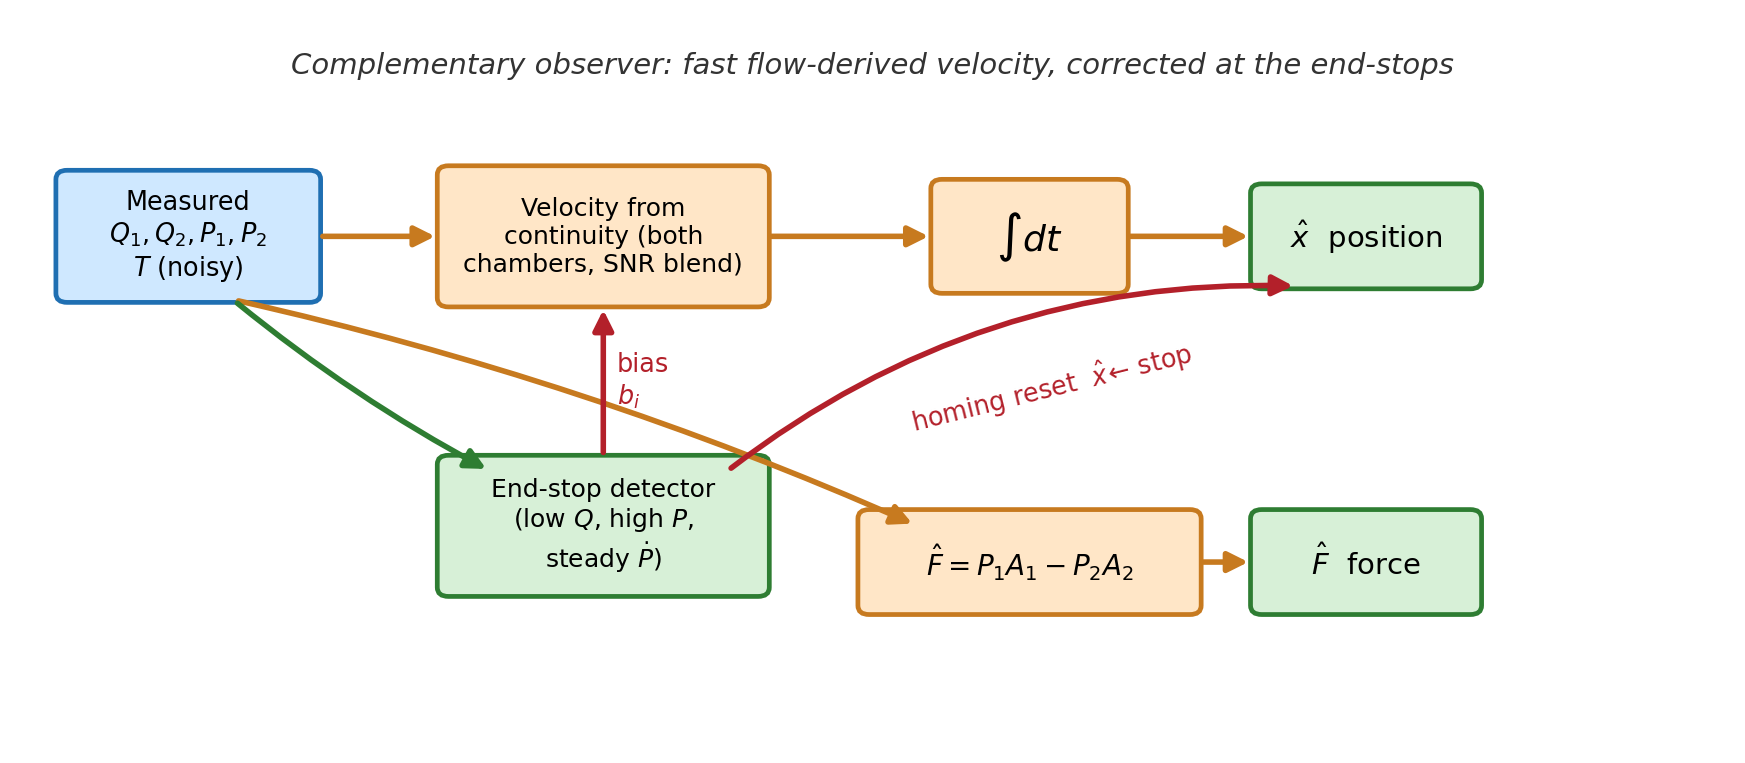
\includegraphics[width=0.92\textwidth]{../figures/fig_observer_block.png}
\caption{The complementary observer as a signal-flow graph. The fast path
(orange) turns measured flows into a velocity and integrates it to position;
pressures give force directly. The end-stop detector supplies the two slow
corrections (red): a \emph{homing reset} that snaps $\hat x$ to the known stop,
and a \emph{bias calibration} $b_i$ that re-zeros the flow meters. The reset is
what bounds integration drift.}
\label{fig:obsblock}
\end{figure*}

The bias $b_i$ is the binding term. We observe it at the end-stops: when the
piston is seated, the true velocity is zero and, in steady state, the measured
flow equals only the known leakage, so $b_1 = Q_1 - q_{\text{leak}}$ and
$b_2 = Q_2 + q_{\text{leak}}$. Seating is detected from low flow plus high
pressure; the bias update is \emph{gated on steady pressure} ($\dot{P}\approx 0$)
so that transient seats, where the bias identity does not hold, are rejected. The
same events pin absolute position (homing), bounding integration drift. Force is
read directly from the measured (filtered) pressures, $F = P_1 A_1 - P_2 A_2$.
Formally this observer is a structurally-reduced realization of an Extended Kalman
Filter on the cylinder state-space model; Appendix~\ref{app:ekf} gives that model,
the EKF recursion and Jacobians, and why the full filter is ill-conditioned for
the stiff hydraulic dynamics (the reason we use the reduced form).

A seated stop gives two \emph{distinct} corrections, easily conflated
(Fig.~\ref{fig:homing}). \textbf{Homing reset} uses the known stop position to
set $\hat{x}\!\leftarrow\!L$ (or $0$): it removes the \emph{accumulated} error
instantly, a vertical drop in the error trace. \textbf{Bias calibration} uses
$v\!=\!0$ to re-identify the flow-meter bias: it removes the \emph{drift source},
reducing the slope at which error grows \emph{between} seats. Reset corrects the
symptom now; calibration slows future growth. Which one dominates depends on how
often the piston seats, examined in Sec.~\ref{sec:results}.

\begin{figure}[!tb]
\centering
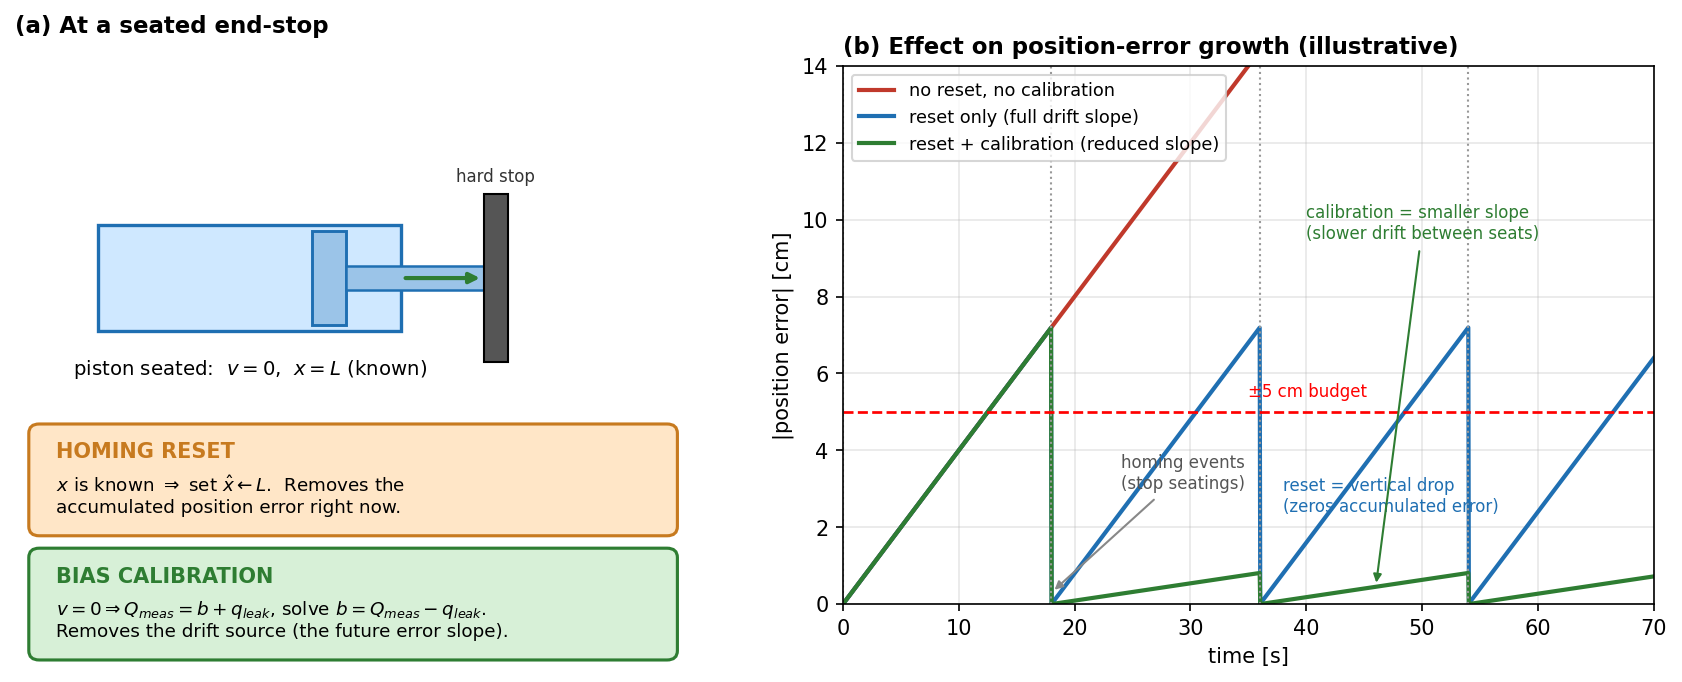
\includegraphics[width=\linewidth]{../figures/fig_homing_concept.png}
\caption{The two end-stop corrections. (a) When seated, position is known
($\Rightarrow$ reset) and velocity is zero so measured flow is bias plus known
leakage ($\Rightarrow$ calibrate the bias). (b) Reset zeros the accumulated error
at each seat (vertical drops); calibration reduces the drift slope between seats.}
\label{fig:homing}
\end{figure}

\section{Experimental Setup}
We sweep six temperatures ($0,10,\dots,50\,$\textdegree C) by eight seeds (each
drawing independent sensor noise/bias and a plant-parameter mismatch), for 48
Monte-Carlo runs. Each run is a $32$-second full-stroke duty cycle at $1$\,kHz,
after a short settling window. The position metric is the maximum absolute error
($\pm 5$\,cm target). For force we use the \emph{operational} metric, the
$99.5$th percentile of absolute error ($\pm 12\,\%$ FS target), and separately
report the transient maximum: a force-from-pressure read-out is unavoidably wrong
for the few milliseconds of a sub-sample pressure reversal, so an instantaneous
max is a transducer property, not an estimator one.

\section{Results}\label{sec:results}
All 48 runs pass. With the realistic plant (friction, valve dynamics, parameter
mismatch) and sensors (bandwidth, delay, drift, saturation), the worst-case
position error across the sweep is $2.58$\,cm (target $5$\,cm) and the worst-case
operational force error is $5.08\,\%$ FS at the $99.5$th percentile (target
$12\,\%$); mean RMS errors are $0.47$\,cm and $1.56\,\%$ FS. The force \emph{max}
reaches $\sim 22\,\%$ FS, but only on $<0.1\,\%$ of samples, confined to the
millisecond pressure reversals at flow direction changes where a delayed,
bandwidth-limited transducer cannot follow a sub-sample pressure swing; this is
a transducer limit, not an estimator one. The headline verdict is in
Table~\ref{tab:results}.

\begin{table}[t]
\caption{Worst-case errors over the 48-run sweep (realistic plant + sensors)}
\label{tab:results}
\centering
\small
\setlength{\tabcolsep}{3.5pt}
\begin{tabular}{@{}lccc@{}}
\toprule
Metric & Target & Worst case & Verdict\\
\midrule
Position error & $\pm 5$\,cm & $2.58$\,cm & \textbf{PASS}\\
Force error (99.5 pct) & $\pm 12\,\%$ FS & $5.08\,\%$ FS & \textbf{PASS}\\
Force error (transient max) & --- & $\sim 22\,\%$ FS & $<0.1\,\%$ samples\\
Temperature & $0$--$50\,$\textdegree C & full range & \checkmark\\
\bottomrule
\end{tabular}
\end{table}

Fig.~\ref{fig:traj} shows a representative run at the hottest, hardest
temperature. The position estimate tracks the truth through the full-stroke sweep
and both end-stop seatings; the error trace stays within about $1.1$\,cm, with
small steps at the homing events where the bias is recalibrated. The force
estimate, read from pressures, sits within a few percent of full scale throughout.

\begin{figure}[!tb]
\centering
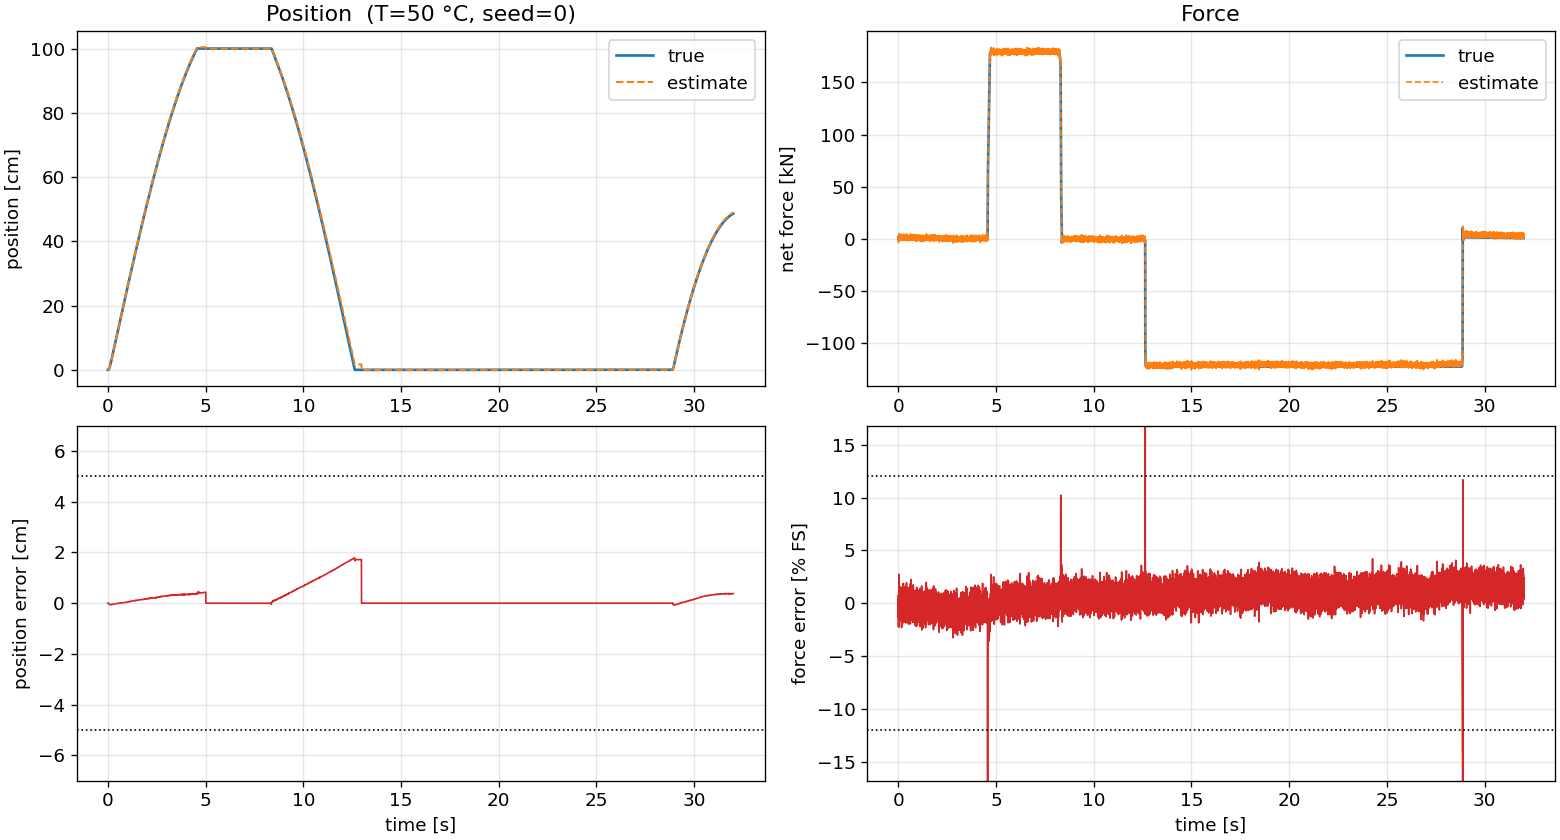
\includegraphics[width=\linewidth]{../figures/fig_trajectory.png}
\caption{Representative run at $50\,$\textdegree C. Left: true vs estimated
position and the error against the $\pm 5$\,cm band (note the bias drift growing
between homing events and resetting at each seat). Right: net force and its error
against the $\pm 12\,\%$ FS band; the brief spikes are the flow-reversal
transients a delayed transducer cannot track. Dotted lines are the limits.}
\label{fig:traj}
\end{figure}

Fig.~\ref{fig:sweep} plots worst-case and mean error against temperature.
Position error is essentially flat across the envelope: the end-stop homing reset
zeros accumulated drift regardless of temperature, and the
temperature-dependent leakage and compressibility corrections handle the rest.
Force error is likewise flat, as expected for a pressure-derived quantity. The
distribution over all 48 runs (Fig.~\ref{fig:hist}) shows every run sitting well
below both limits, with no temperature-correlated tail. The full ensemble of
error-vs-time traces (Fig.~\ref{fig:mc}) makes the spread explicit: every run's
position error stays inside the $\pm 5$\,cm band throughout, with the largest
excursions during the mid-stroke window between homing events, while the
force-error traces form a tight band near $\pm 4\,\%$ FS.

\begin{figure}[!tb]
\centering
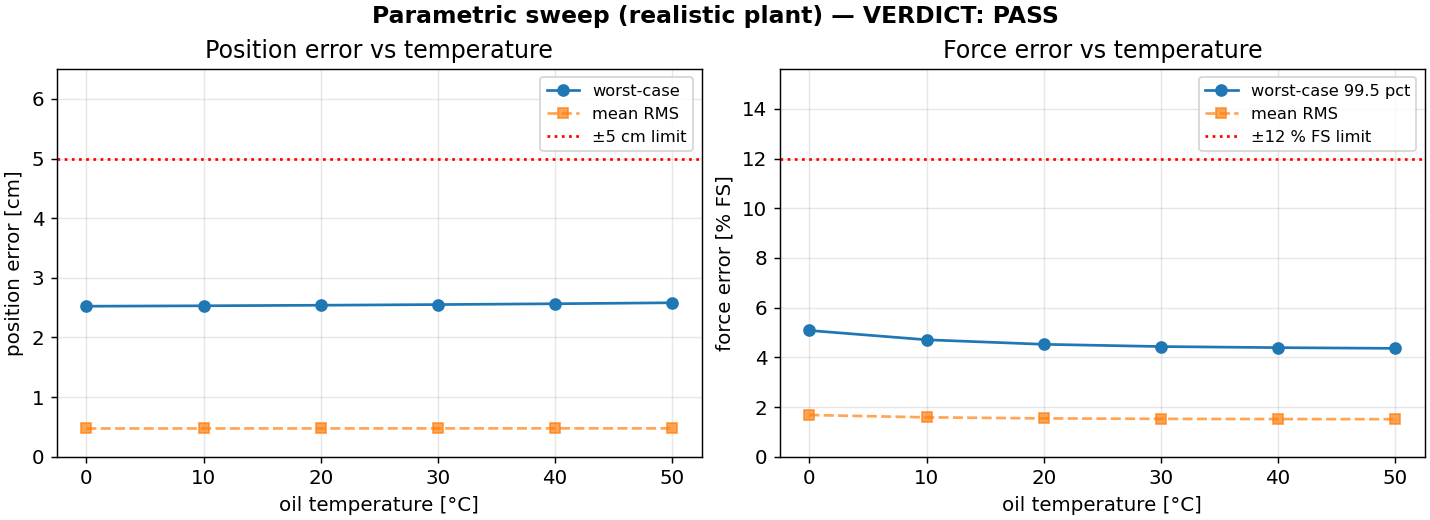
\includegraphics[width=\linewidth]{../figures/fig_sweep.png}
\caption{Worst-case and mean error versus oil temperature. Both metrics stay flat
and far below the limits across $0$--$50\,$\textdegree C.}
\label{fig:sweep}
\end{figure}

\begin{figure}[!tb]
\centering
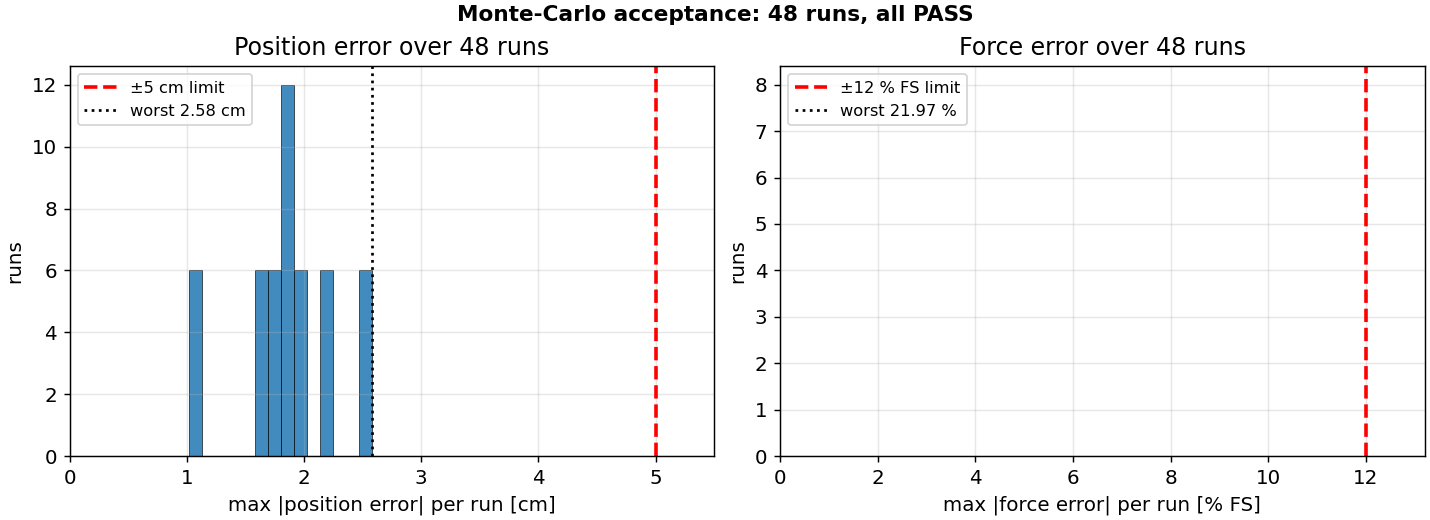
\includegraphics[width=\linewidth]{../figures/fig_error_hist.png}
\caption{Error distributions over all 48 Monte-Carlo runs. Every run is inside
both acceptance limits (red dashed); worst cases marked.}
\label{fig:hist}
\end{figure}

\begin{figure}[!tb]
\centering
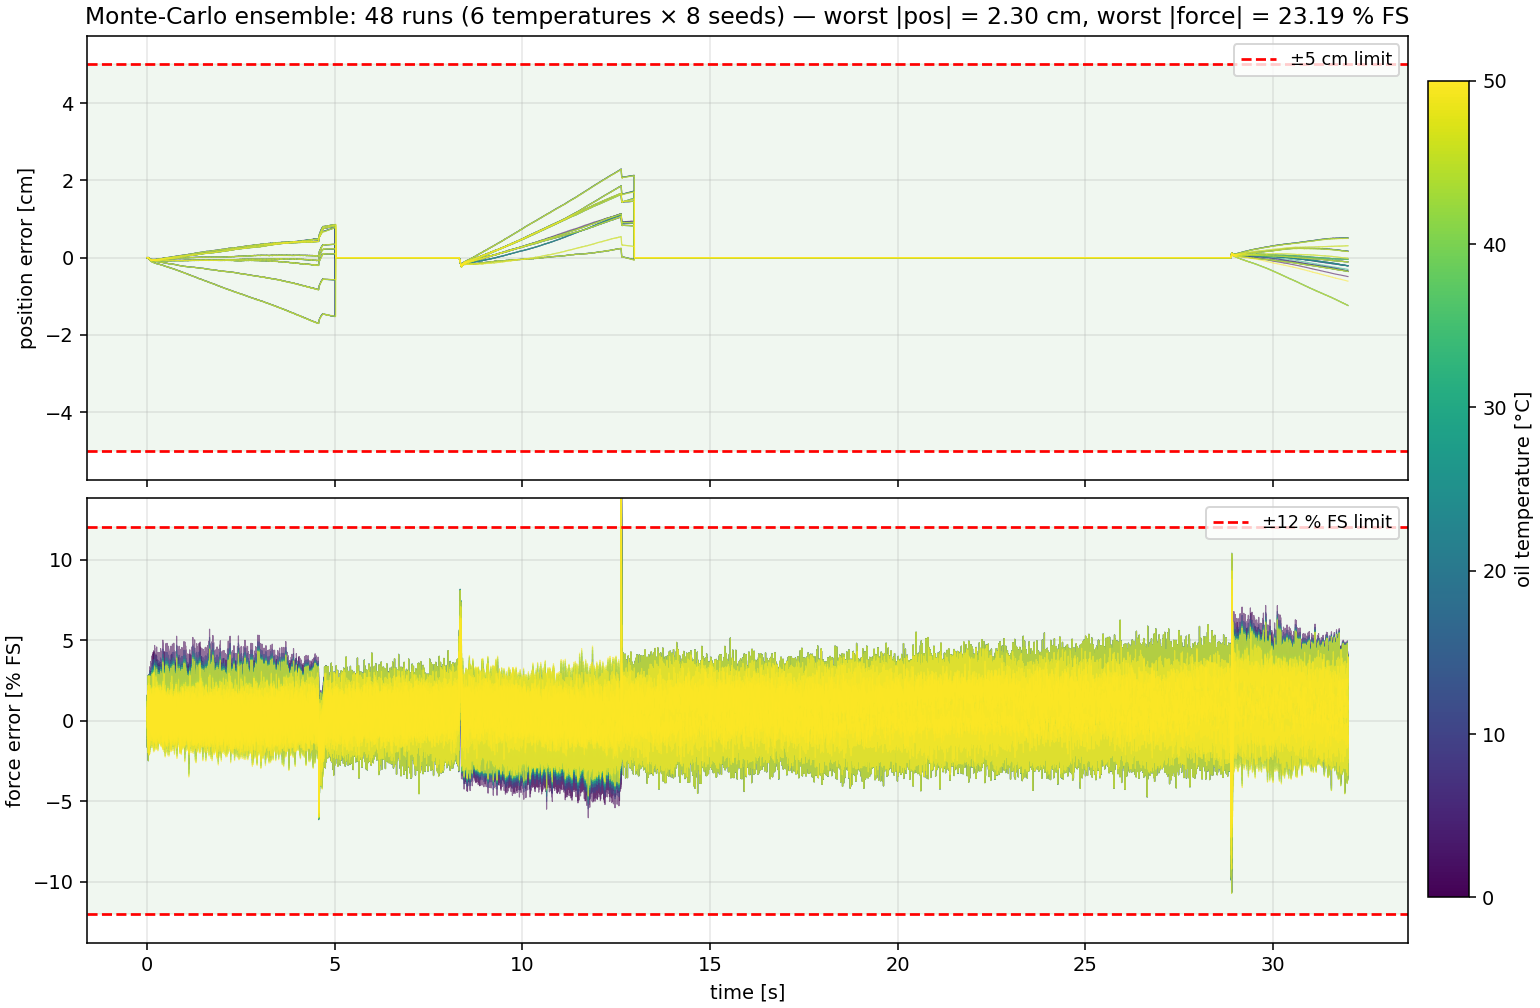
\includegraphics[width=\linewidth]{../figures/fig_mc_ensemble.png}
\caption{Monte-Carlo ensemble: all 48 error-vs-time traces overlaid, coloured by
oil temperature, against the acceptance bands (green shading, red dashed limits).
Top: position error; bottom: net-force error. The position spread stays inside
$\pm 5$\,cm with the largest excursions mid-stroke between homing events; the
force band sits near $\pm 4\,\%$ FS.}
\label{fig:mc}
\end{figure}

\subsection{Ablations: which mechanism matters}\label{sec:ablation-finding}
Turning observer features off one at a time (Fig.~\ref{fig:ablation}) shows the
result is not generic. Disabling end-stop \emph{homing} pushes the worst case to
$4.9$\,cm (at the edge of target), so the homing reset is the primary
load-bearing mechanism under this frequently-seating duty cycle. The
\emph{steady-pressure gate} is what makes bias calibration safe: removing it
nearly triples the error to $7.3$\,cm (fail), because ungated transient seats
inject compressibility flow as false bias. Notably, removing bias calibration
\emph{entirely} leaves the worst case unchanged ($2.2$\,cm): under frequent
seating the homing reset dominates, and calibration matters mainly for large bias
or sparse homing. The leakage, compressibility, single-chamber and temperature
variants stay near $2$--$2.5$\,cm: second-order refinements.

\begin{figure}[!tb]
\centering
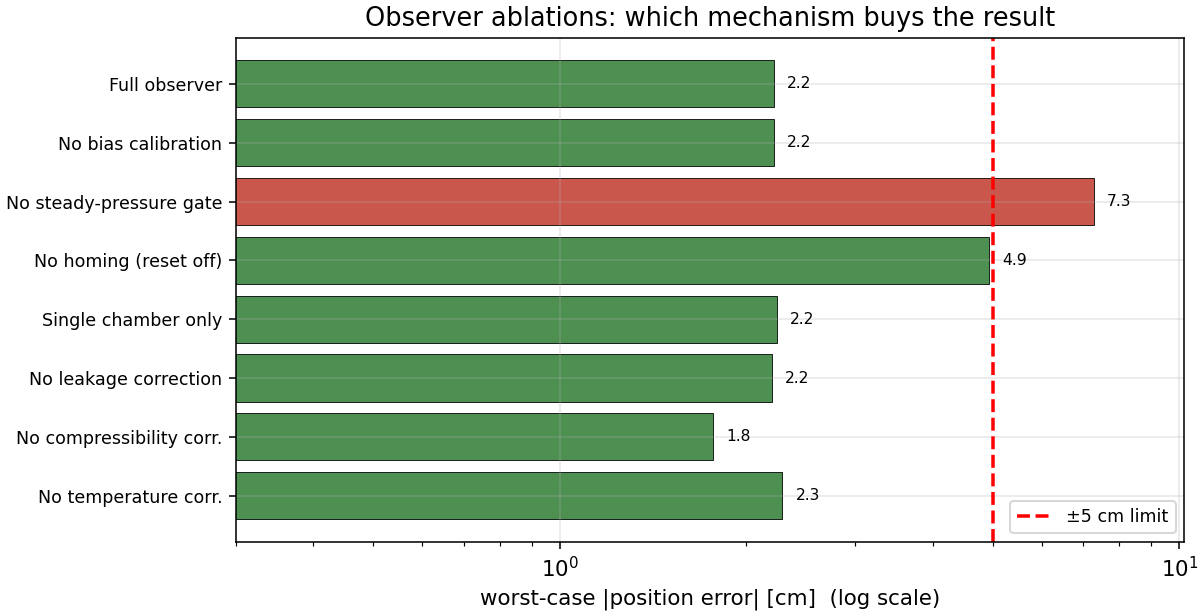
\includegraphics[width=\linewidth]{../figures/fig_ablation.png}
\caption{Observer ablations (worst case over a temperature/seed subset, log
scale). Removing the steady-pressure gate or the homing reset is what breaks the
result; the physical corrections are minor.}
\label{fig:ablation}
\end{figure}

\subsection{How often must the actuator home, and why?}
The duty cycle seats a stop every half reference-period, so we sweep the
reference frequency to vary the interval between homing events, $8$ seeds per
point, in three observer modes (Fig.~\ref{fig:stress}). The result both gives a
design rule and settles which mechanism is load-bearing. For the full observer
the median error rises with interval and the $\pm 5$\,cm budget holds in the
median while the actuator seats a stop roughly every $\lesssim 30$\,s; the
upper-quartile band reaches the limit nearer $\lesssim 20$\,s, so $\sim 20$\,s is
a reasonable distributional guideline. It is not a hard guarantee: individual
unlucky mismatch draws can exceed $\pm 5$\,cm even at shorter intervals, so a
safety-critical use would need a tail-reliability budget. Crucially, \emph{reset-only}
(calibration disabled) tracks the full observer almost exactly across the whole
range, whereas \emph{calibration-only} (homing reset disabled) is worse at every
interval and diverges once seating is sparse. So the \textbf{homing reset is the
load-bearing mechanism}: it zeros error from \emph{all} sources (bias, mismatch,
noise) at each seat, while bias calibration only removes the flow-meter-bias part
of the between-seat slope and cannot bound dead-reckoning drift on its own.
Calibration is a useful refinement (it extends the usable interval modestly), not
the foundation.

\begin{figure}[!tb]
\centering
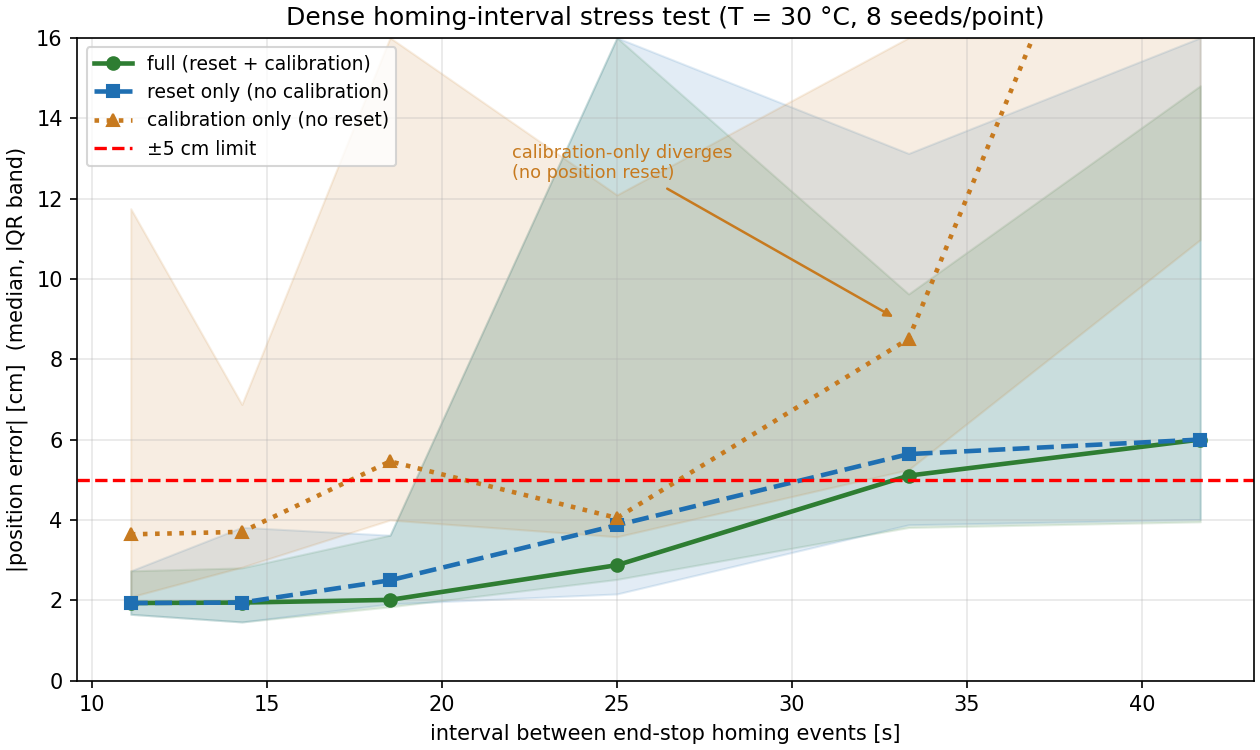
\includegraphics[width=\linewidth]{../figures/fig_stress_dense.png}
\caption{Dense homing-interval stress test (median, inter-quartile band; 8 seeds).
Full ($\bullet$) and reset-only ($\blacksquare$) nearly coincide and hold
$\pm 5$\,cm out to $\sim 30$\,s; calibration-only ($\blacktriangle$, no position
reset) is worse everywhere and diverges. The homing reset, not the bias
calibration, is what bounds the error.}
\label{fig:stress}
\end{figure}

\subsection{Operating envelope: supply pressure and cylinder size}
Holding the duty cycle, we sweep the two parameters a deployment varies most:
supply pressure and bore. \textbf{Pressure} (Fig.~\ref{fig:pressure}): position
error is flat from $60$--$280$\,bar, because the flow-continuity estimate barely
uses pressure. Force error instead scales like $1/P_{\text{supply}}$ when the
transducer full scale is fixed (a $250$-bar transducer gives $\sim 9.5\,\%$ FS at
$60$\,bar, near the limit), but is flat once the transducer is matched to the
supply. Low-pressure operation is thus harder for force only through transducer
SNR, a sizing choice, not an estimator limit. Even the deeper low-pressure
physics leaves position unmoved: adding an entrained-air bulk modulus $\beta(P)$
that collapses below $\sim 50$\,bar (Fig.~\ref{fig:betaP}) changes position
negligibly, and a naive constant-$\beta$ observer matches a pressure-aware one,
because the flow channel is $\beta$-insensitive.

\textbf{Size} (Fig.~\ref{fig:bore}): across ISO bores $63$--$160$\,mm (area-
similarity scaling) position error is flat at $\sim 2.3$\,cm and force at
$\sim 2.6\,\%$ FS, \emph{provided the flow meter is sized to the cylinder}; a
fixed meter fails at both ends (saturation for large bores, noise floor for
small). The estimation itself is therefore robust across the envelope, subject to
two clean sensor-sizing rules: \textbf{size the pressure transducer to the supply
(for force) and the flow meter to the cylinder area (for position)}.

\begin{figure}[!tb]
\centering
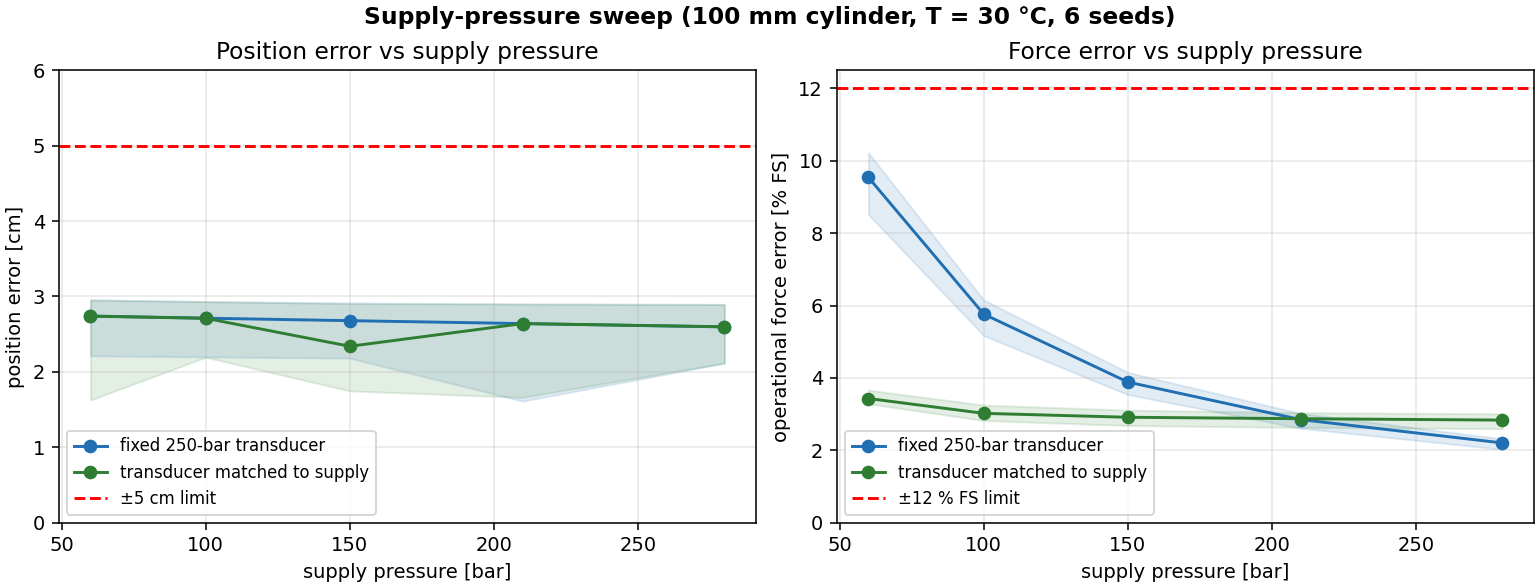
\includegraphics[width=\linewidth]{../figures/fig_pressure_sweep.png}
\caption{Supply-pressure sweep ($100$\,mm cylinder). Position is flat; force error
rises as $1/P$ with a fixed $250$-bar transducer but is flat with a transducer
matched to the supply.}
\label{fig:pressure}
\end{figure}

\begin{figure}[!tb]
\centering
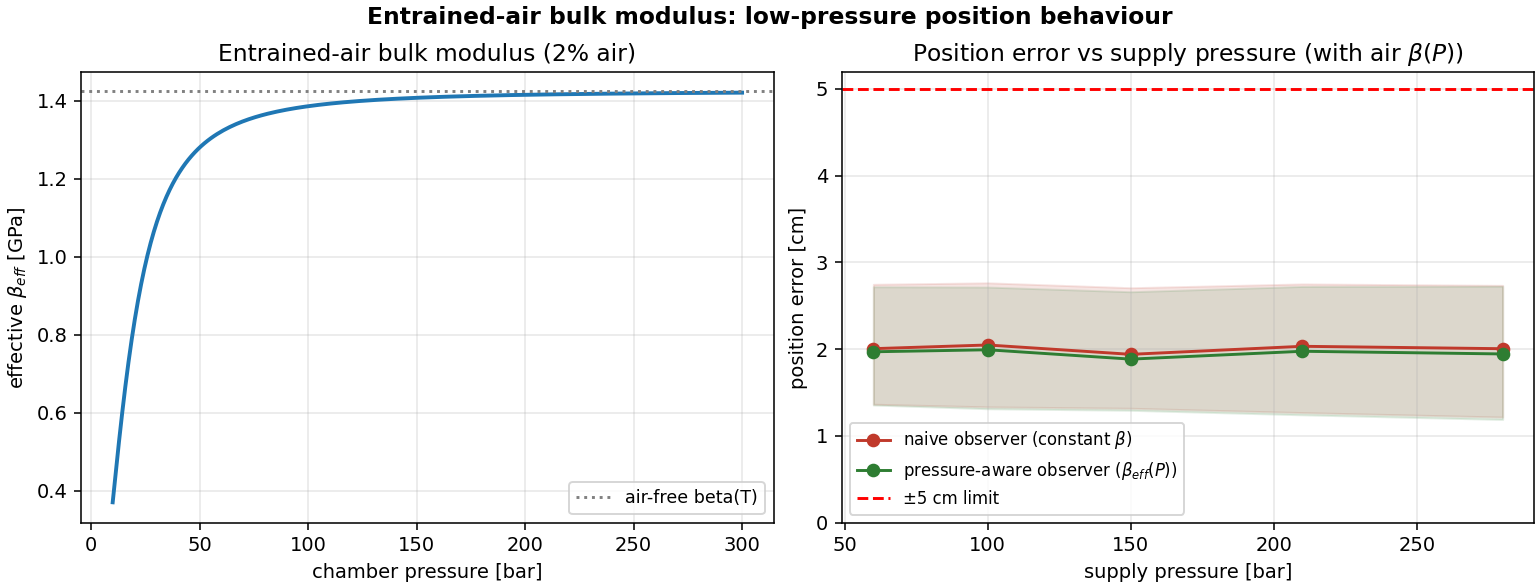
\includegraphics[width=\linewidth]{../figures/fig_betaP.png}
\caption{Entrained-air bulk modulus. Left: $\beta_{eff}(P)$ collapses below
$\sim 50$\,bar. Right: yet position error stays flat and a naive constant-$\beta$
observer matches a pressure-aware one, because the flow-based position estimate
is $\beta$-insensitive.}
\label{fig:betaP}
\end{figure}

\begin{figure}[!tb]
\centering
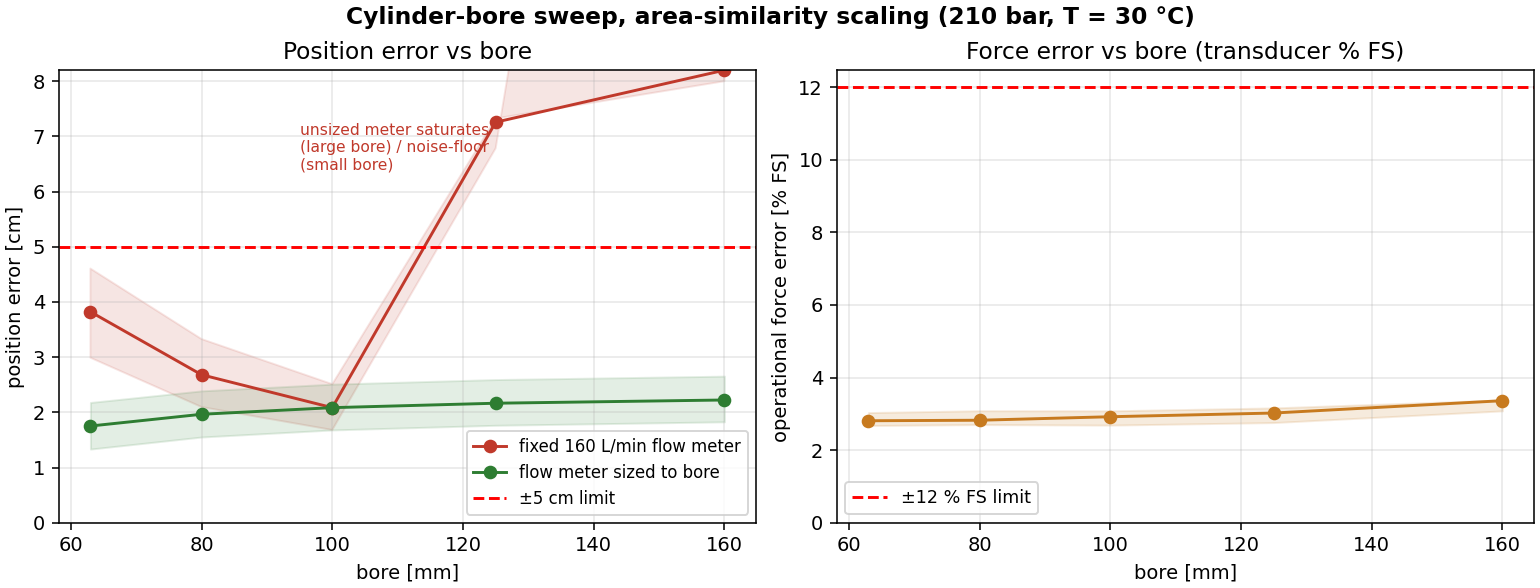
\includegraphics[width=\linewidth]{../figures/fig_bore_sweep.png}
\caption{Bore sweep ($63$--$160$\,mm, area-similarity scaling). With a flow meter
sized to the cylinder, position and force are flat across sizes; a fixed
$160$\,L/min meter saturates at large bores and is noise-floor-limited at small.}
\label{fig:bore}
\end{figure}

\subsection{Hose length: how far can the sensors sit from the cylinder?}
\label{sec:hose}
A real installation places the transducers at the valve manifold and runs a hose
to the cylinder (Sec.~\ref{sec:plant}), so the sensed pressure and flow are
\emph{upstream} of a line loss. We sweep the hose length from $0.5$ to $25$\,m
(standard $3/4$\,in.\ mobile-hydraulics pressure hose) at three oil temperatures
and ask how this degrades each estimate (Fig.~\ref{fig:hose}).

The two channels respond oppositely, and the reason is instructive.
\textbf{Position is almost length-independent} (flat at $\sim\!2.9$\,cm out to
$25$\,m): the friction drop along the hose does not destroy flow---in steady
state the flow that enters the hose at the manifold is the flow that reaches the
cylinder---so integrating the measured flow still recovers the stroke, and the
only residual is the small transient stored in the line compliance.
\textbf{Force degrades with length}, because force is read straight off the
manifold pressure, which exceeds the true cylinder pressure by the line drop
$\Delta p = Q/K_c$. That drop grows with length and, through the viscosity in
$K_c\!\propto\!1/\mu$, with \emph{cold} oil: at $50$\,\textdegree C the force
error stays near $5\,\%$ FS even at $25$\,m, but at $0$\,\textdegree C it crosses
the $\pm 12\,\%$ FS limit at $\sim\!15$\,m. The worst case is therefore a long
hose at cold start---a concrete, physically-grounded design rule: \emph{position
tolerates an arbitrarily distant manifold, but the force specification sets a
maximum hose length that shortens as the oil gets colder}. The fix, if a longer
run is unavoidable, is to subtract a modelled $\Delta p(Q,T)$ from the measured
pressure---the same line model used here, run forward. Figure~\ref{fig:transient}
shows the mechanism directly in a single Hopsan run: a standing offset between the
measured (manifold) and true (cylinder) pressures---the force-channel error---plus
a sharp transient at each direction reversal.

\begin{figure}[!tb]
\centering
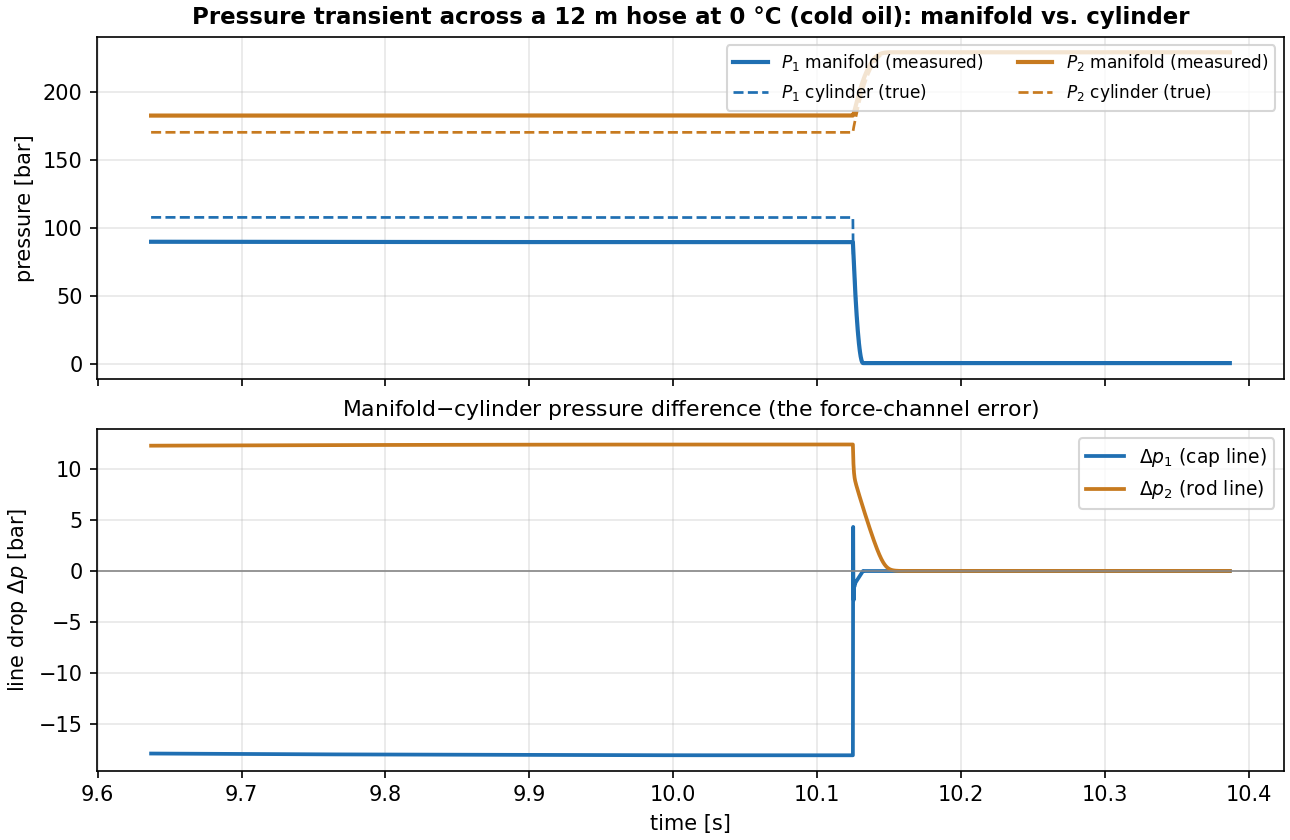
\includegraphics[width=\linewidth]{../figures/fig_transient.png}
\caption{Hopsan pressure transient across a $12$\,m hose at $0$\,\textdegree C.
Top: measured manifold pressures (solid) sit $\sim\!12$--$18$\,bar off the true
cylinder pressures (dashed)---a force read directly from the manifold inherits
this gap. Bottom: the line drop $\Delta p$ for each chamber, steady between events
and spiking at the reversal near $10.1$\,s.}
\label{fig:transient}
\end{figure}

\begin{figure}[!tb]
\centering
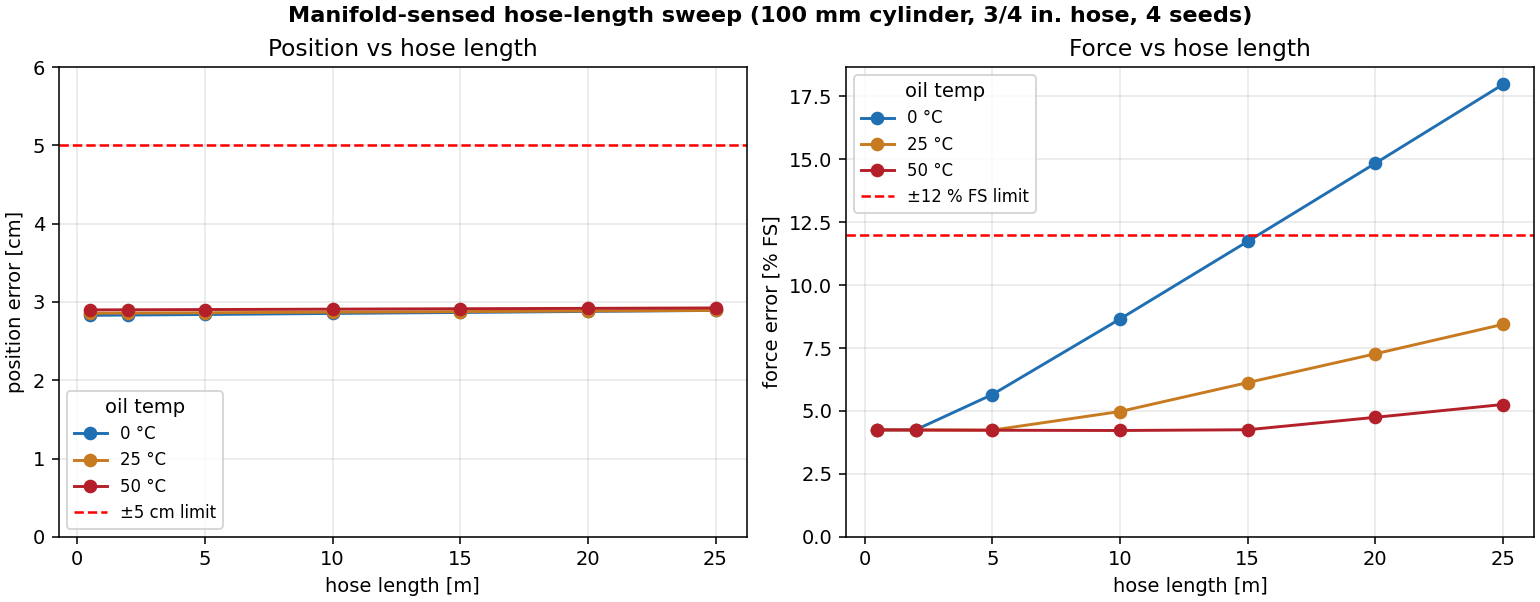
\includegraphics[width=\linewidth]{../figures/fig_hose_sweep.png}
\caption{Hose-length sweep with manifold-located sensors ($100$\,mm cylinder,
$3/4$\,in.\ hose). Position (left) is nearly length-independent because flow is
conserved along the hose; force (right) carries the full line-loss offset, which
grows with length and with cold oil (higher viscosity), crossing $\pm 12\,\%$ FS
near $15$\,m at $0$\,\textdegree C.}
\label{fig:hose}
\end{figure}

\subsection{Open-loop excitation at bench scale}\label{sec:bench}
All results so far drive the plant with a position controller. To check that the
estimator does not secretly lean on the loop, we replaced the controller with an
\emph{open-loop} sinusoidal spool command (a separate Hopsan model variant in
which the valve input is wired directly to the signal generator rather than to the
PI controller) and re-scaled the rig to a small laboratory cylinder: $40$\,mm
bore, $16$\,mm rod, $0.1$\,m stroke, $3$\,kg load, $100$\,bar supply, with the
flow meter and transducer sized to the bench ($20$\,L/min, $120$\,bar). A
benchtop rig plumbs the cylinder directly at the valve block, so unlike the
manifold-sensed industrial case (Sec.~\ref{sec:hose}) the sensors sit at the
cylinder and this variant is line-free. Because the stroke is now $0.1$\,m, the
$\pm5$\,cm position target is expressed as its geometric equivalent,
$\pm5\,\%$ of stroke. Across $0$--$50$\,\textdegree C and
eight mismatch seeds the estimator holds \textbf{$4.5\,\%$ of stroke worst-case
position} and \textbf{$4.9\,\%$ FS force} (Fig.~\ref{fig:bench}), meeting both
targets without a controller in the loop.

Reaching that number required fixing a failure mode that only \emph{open-loop}
excitation exposes, and which is instructive about what the homing reset actually
depends on. The reset must decide \emph{which} stop a seated piston rests against.
Under closed-loop control the answer is trivial: the controller pushes the piston
into the commanded stop, so the pressurized chamber names the stop. Under open-loop
excitation it is not, because near a stop the spool sine keeps cycling and both
chambers can dead-head close to supply pressure. A naive ``chamber with the higher
pressure wins'' rule then mis-identifies the stop on a few-bar difference, and---
since the cap area exceeds the rod area---a force-balance rule ($P_1A_1\!>\!P_2A_2$)
is no better, biasing every dead-headed seat toward ``extended.'' The pressures
simply do not carry the stop identity when both chambers are pressurized. The
robust, still-sensorless cue is \emph{direction of travel}: the piston rests
against whichever stop it last moved toward. We latch the sign of the displacement
accumulated over each off-stop excursion (committing it only past $30\,\%$ of
stroke, so dwell jitter---which can flip the instantaneous velocity sign, the more
so at $50$\,\textdegree C where leakage corrupts the velocity estimate---cannot
flip the latch). With the travel-direction cue the divergent seeds vanish at every
temperature. The closed-loop results above are unchanged by this modification
(direction of travel and pressurized chamber agree when a controller holds the
stop), so it is a strict generalization. The lesson reinforces
Sec.~\ref{sec:ablation-finding}: homing is load-bearing, but only if the reset can
reliably tell the stops apart---and outside closed-loop control that identification
must come from motion history, not instantaneous pressure.

\begin{figure}[!tb]
\centering
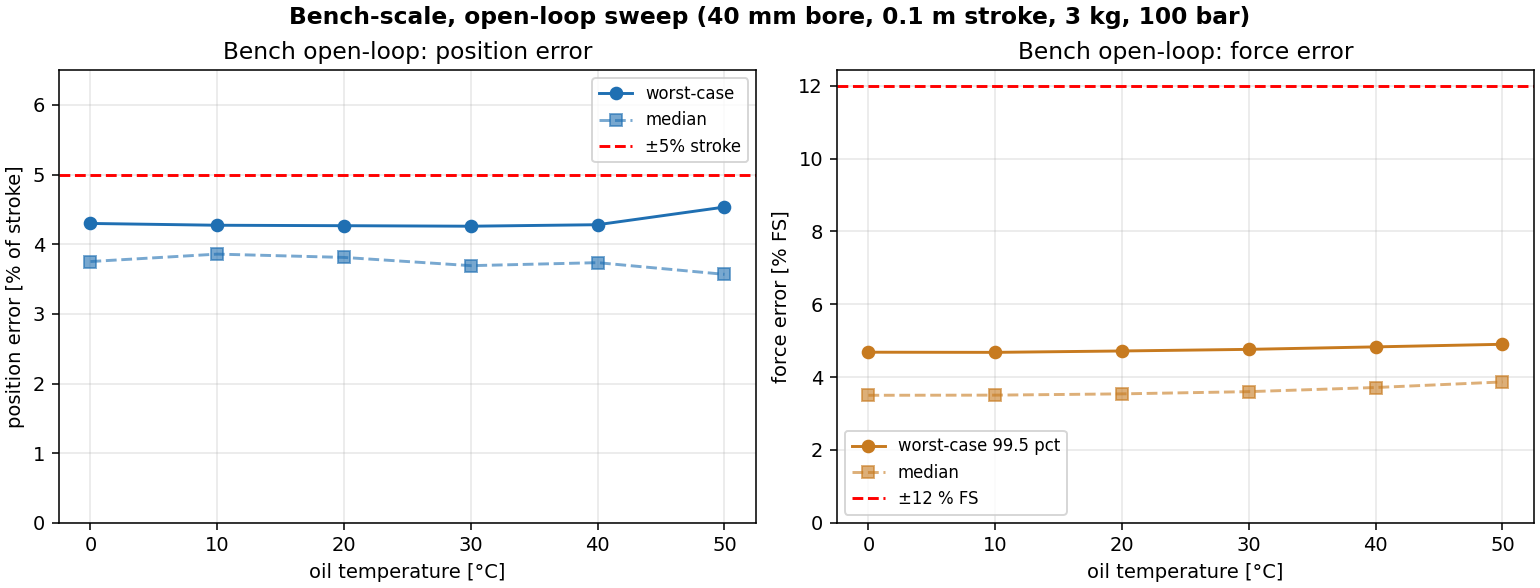
\includegraphics[width=\linewidth]{../figures/fig_bench_sweep.png}
\caption{Bench-scale, \emph{open-loop} sweep ($40$\,mm bore, $0.1$\,m stroke,
$3$\,kg, $100$\,bar; no position controller). Worst-case position stays at
$\sim4.3\,\%$ of stroke and force below $5\,\%$ FS across $0$--$50$\,\textdegree C,
once the homing reset identifies the seated stop from direction of travel rather
than from chamber pressure.}
\label{fig:bench}
\end{figure}

\subsection{Comparison with a well-scaled EKF}\label{sec:ekf}
We implemented the Extended Kalman Filter of Appendix~\ref{app:ekf} as a direct
competitor, with the engineering needed to make it run on this stiff plant:
non-dimensionalized states (fixing the conditioning that made an earlier
prototype diverge), semi-implicit integration for the fast pressure mode, both
pressures \emph{and} both flows as measurements, an end-stop force in the model,
and seated pseudo-measurements ($x{=}$stop, $v{=}0$) that are the filter's analog
of homing. It is now numerically stable and converges. Table~\ref{tab:ekf} and
Fig.~\ref{fig:ekf} give the head-to-head on identical truth and measurements.

\begin{table}[t]
\caption{EKF vs complementary observer (worst case over 24 runs)}
\label{tab:ekf}
\centering
\small
\begin{tabular}{@{}lcc@{}}
\toprule
Metric & Observer & EKF\\
\midrule
Position error, full run (cm) & $2.58$ & $21.5$\\
Position error, post-convergence (cm) & $2.58$ & $3.9$\\
Position RMS (cm) & $0.65$ & $3.6$\\
Force error, 99.5 pct (\% FS) & $5.08$ & $4.90$\\
Covariance calibration (within $2\sigma$) & --- & $82\,\%$\\
\bottomrule
\end{tabular}
\end{table}

The force estimates are comparable (the EKF's is marginally better, coming from
its filtered pressure state). On position, though, the observer is clearly
better and more robust: the EKF lags the first stroke until its first homing and
shows larger mid-stroke and reversal excursions for unfavorable mismatch draws,
and its $2\sigma$ band is optimistic ($82\,\%$ coverage versus the ideal
$95\,\%$). The observer's algebraic velocity and held-bias structure are simply
better matched to a plant where absolute position is weakly observable and the
dynamics are stiff. The EKF's one real advantage is the covariance it carries
(the shaded band in Fig.~\ref{fig:ekf}); making that both tight and
well-calibrated would need further tuning. This is consistent with the ablation:
the homing reset bounds position, and both estimators depend on it.

\begin{figure}[!tb]
\centering
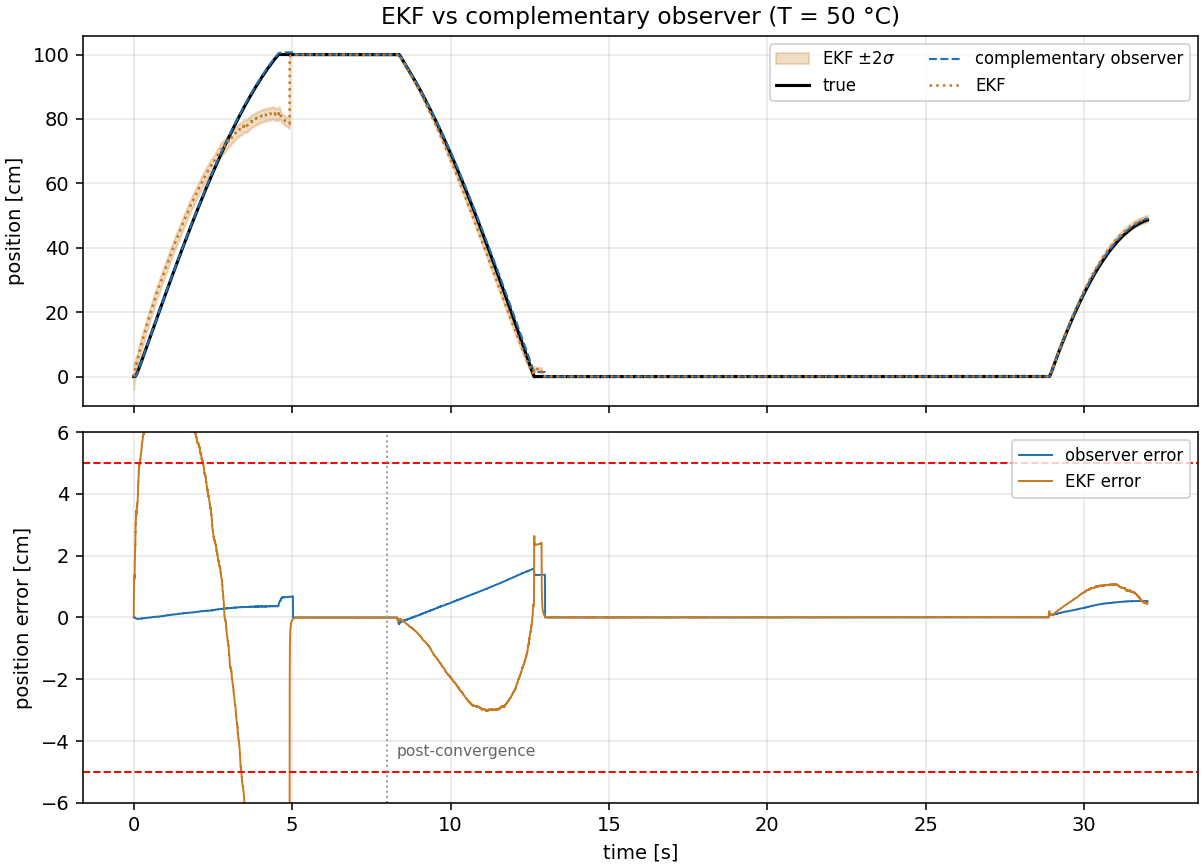
\includegraphics[width=\linewidth]{../figures/fig_ekf_compare.png}
\caption{EKF vs complementary observer on one run ($50\,$\textdegree C). Top:
position, with the EKF $\pm 2\sigma$ band. Bottom: errors against the $\pm 5$\,cm
band. The EKF lags the first ramp until its first homing and has larger
transients; the observer stays tighter throughout.}
\label{fig:ekf}
\end{figure}

\subsection{External validation against a physical rig}\label{sec:zhou}
Our results are simulation-based by construction, so it matters that an
independent \emph{experimental} study reaches a compatible conclusion on real
hardware. Zhou et al. \cite{zhou2022pressure} reconstruct the position of a
fully-mechanized mining support cylinder ($180$\,mm bore, $120$\,mm rod, $900$\,mm
stroke, $500$\,kg, water-glycol emulsion) by the same flow-integration principle,
predicting flow from the inlet/outlet pressures through a throttle law and
integrating $Q/A$. On a $400$\,L/min test platform they sweep the supply from $5$
to $31$\,MPa and report the relative error between predicted and measured flow
(their Table 8); since position is the time integral of $Q/A$, that
flow-coincidence error is, to first order, their position error.

We reconfigured our Hopsan plant and observer to their rig---geometry, load,
emulsion bulk modulus ($2.01$\,GPa), Coulomb/static friction ($7$/$10.5$\,kN), a
$0$--$40$\,MPa transducer and a $400$\,L/min flow meter---and swept the same
supply pressures, with the plant bulk modulus following the entrained-air
$\beta_{\text{eff}}(P)$ model so that the real low-pressure softening they invoke
is present. The driven stroke reaches $296$\,L/min peak flow, matching their
measured range. Figure~\ref{fig:zhou} and Table~\ref{tab:zhou} compare the two.

\begin{table}[t]
\caption{Position-estimation error vs.\ the experiment of \cite{zhou2022pressure}}
\label{tab:zhou}
\centering
\footnotesize
\begin{tabular}{cccc}
\hline
Supply & Zhou et al.\ exp.\ & This work & This work \\
{[MPa]} & (flow err., range) & (pos., median) & (pos., worst) \\
\hline
 5 & $12.1$--$20.1\,\%$ & $2.4\,\%$ & $3.0\,\%$ \\
10 & $0.0$--$13.8\,\%$  & $2.4\,\%$ & $3.1\,\%$ \\
15 & $0.0$--$0.5\,\%$   & $2.4\,\%$ & $3.1\,\%$ \\
20 & $0.5$--$3.2\,\%$   & $2.4\,\%$ & $3.1\,\%$ \\
25 & $0.5$--$4.8\,\%$   & $2.4\,\%$ & $3.1\,\%$ \\
30 & $1.4$--$4.9\,\%$   & $2.3\,\%$ & $3.0\,\%$ \\
\hline
\end{tabular}
\end{table}

Two things follow. \textbf{At and above $15$\,MPa} the experiment and our observer
agree closely---both sit below $5\,\%$, ours at $2.4$--$3.2\,\%$ of stroke, well
inside their experimental band---so the core mechanism is corroborated on real
hardware at the pressures mining supports actually run. \textbf{Below $10$\,MPa}
the comparison is more interesting: Zhou et al.\ degrade to $12$--$20\,\%$, and
attribute it explicitly to the bulk modulus varying in the low-pressure region
(``the elastic modulus is equivalent to a constant when system pressure is above
$10$\,MPa''). That is precisely the entrained-air $\beta_{\text{eff}}(P)$ physics
of Sec.~\ref{sec:results} (Fig.~\ref{fig:betaP}). Our observer, however, stays
flat at $\sim\!2.4\,\%$ there, because it carries the compressibility term
$(V/\beta)\dot{P}$ explicitly and re-zeros at end-stops, whereas a steady-state
pressure-to-flow fit cannot separate compression flow from motion flow when the
fluid is soft. The experiment thus both validates our high-pressure numbers and
independently confirms the low-pressure mechanism we model---while highlighting
why a compressibility-aware, homing observer is more robust there than a
steady-state flow fit. The residual experimental scatter at $5$--$10$\,MPa also
reflects flow-meter response lag at low flow, a sensor effect orthogonal to the
estimator. (Force is not reported in \cite{zhou2022pressure}; our force error
rises at low supply only through fixed-transducer SNR, the $1/P$ effect of
Fig.~\ref{fig:pressure}, reaching $\sim\!22\,\%$ FS at $5$\,MPa with a $40$\,MPa
transducer and falling below $5\,\%$ once the supply exceeds $20$\,MPa.)

\begin{figure}[!tb]
\centering
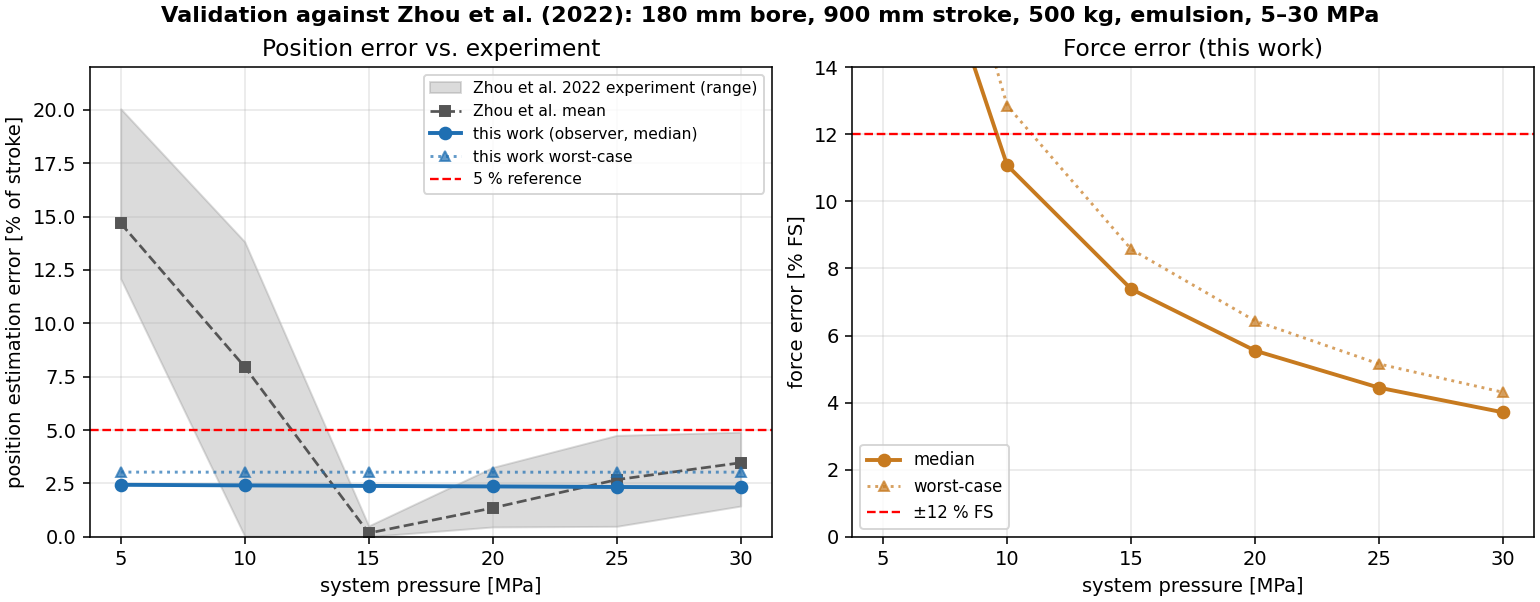
\includegraphics[width=\linewidth]{../figures/fig_zhou_validation.png}
\caption{Validation against the physical experiment of \cite{zhou2022pressure}
(180\,mm bore, 900\,mm stroke, 500\,kg, emulsion). Left: our observer's position
error (blue) against their measured flow-coincidence error envelope (grey). The
two agree below $5\,\%$ above $15$\,MPa; below $10$\,MPa the experiment degrades
with the softening bulk modulus while the compressibility-aware, homing observer
stays flat. Right: our force error, which rises at low supply only through fixed-
transducer SNR.}
\label{fig:zhou}
\end{figure}

\section{Discussion}
The result rests on one mechanism. Position from flow integration is
\emph{bias-limited}, not noise-limited: zero-mean flow noise integrates to a small
random walk, but a constant flow-meter offset integrates to unbounded drift. Early
in the study, runs with unlucky bias draws produced $13$\,cm of drift during a
long mid-stroke excursion. The fix was not a better filter but recognising that
the bias is directly observable wherever the piston seats a hard stop, and gating
that calibration on steady pressure so transient seats do not corrupt it. The
ablation (Fig.~\ref{fig:ablation}) confirms this: the gate and the homing reset
are what hold the result; the leakage/compressibility/temperature corrections are
refinements. With realistic per-run parameter mismatch the residual position
error rises only from $\sim 2.1$ to $\sim 2.9$\,cm, so the scheme tolerates the
$10$--$20\,\%$ fluid-parameter uncertainty a field estimator would face.

Force, being a direct pressure read-out, is accurate in operation
($99.5$th-percentile $\sim 4\,\%$ FS) but is \emph{transducer-limited at fast
reversals}: when a chamber drains toward cavitation in under a sample, a delayed
bandwidth-limited sensor reports a stale value and the instantaneous force is
briefly wrong. This is a real measurement limit, and a force-from-pressure scheme
inherits it.

The practical reading is that for this class of actuator, periodic end-stop
homing converts a hard absolute-position problem into a bounded-drift problem that
cheap pressure and flow sensing can solve to a few centimetres. The stress test
(Fig.~\ref{fig:stress}) makes the dependence quantitative: the budget holds only
while the actuator seats a stop often enough. A process that parks mid-stroke for
long periods would drift past target and would need an independent absolute
reference.

\section{Limitations}
This is a simulation spike, not a hardware validation. The plant now includes
Coulomb/stiction friction, finite valve bandwidth and per-run parameter mismatch,
and the sensors include bandwidth, delay, drift and saturation; but air
entrainment, valve hysteresis/deadband, structural compliance and sensor failure
modes are still simplified or absent, and the TLM solver is a validated model,
not measured hardware. Temperature is a steady per-run constant; within-stroke
thermal transients are out of scope. The envelope now spans $60$--$280$\,bar and
$63$--$160$\,mm bore, but still one duty-cycle family that periodically seats
stops. The force result remains, fundamentally, pressure sensing rather than a
hard inference problem, and its accuracy degrades at fast pressure reversals.

\section{Conclusion}
Within a 0--50\,\textdegree C envelope, with realistic sensor non-idealities,
Coulomb friction, valve dynamics and $10$--$20\,\%$ plant/estimator parameter
mismatch, a double-acting hydraulic cylinder modelled in Hopsan can be
position-estimated to $2.58$\,cm and force-estimated to $5.08\,\%$ of full scale
(operationally) without a position sensor, inside the $\pm 5$\,cm and $\pm 12\,\%$
targets, using flow-continuity velocity with end-stop bias calibration and
pressure-derived force. A three-mode stress test identifies the end-stop
\emph{homing reset} as the load-bearing mechanism (it zeros error from all
sources at each seat); bias calibration is a secondary refinement that cannot
bound drift alone, and the $\pm 5$\,cm budget yields a concrete homing-interval
design rule. The
harness, with Hopsan as the truth plant feeding a sensor and observer pipeline,
is reusable for sharper questions: drift between homing events, extended Kalman
variants with covariance bounds, and a hardware bridge through Hopsan's FMU
export. Detailed equations, parameter tables, and the full human/AI session log
are in the appendix.

\section*{Acknowledgements}
This work, including the simulation harness, the Hopsan integration and the
writing, was carried out with the assistance of Anthropic's Claude (Claude Code),
used both for running the experiments and for drafting this paper. All design
decisions, target setting and verification were directed by the author.

\bibliographystyle{IEEEtran}
\bibliography{refs}

\appendices
\section{Full Parameter Set}\label{app:params}
Table~\ref{tab:fullparams} lists every parameter, complementing the abbreviated
Table~\ref{tab:sensors}. The temperature curves are
$\beta_e(T)=\beta_0\,[1+k_\beta(T-T_0)]$ with $\beta_0=1.5$\,GPa, $T_0=20$,
$k_\beta=-0.005\,$\textdegree C$^{-1}$ (clamped at $0.3$\,GPa);
$\mu(T)=\mu_{40}\exp\!\big(B(1/T_K-1/T_{K,40})\big)$ (Vogel-like) with
$\mu_{40}=41$\,mPa\,s and $B=3100$\,K; and
$C_{\text{leak}}(T)=C_0\,\mu_{40}/\mu(T)$ with $C_0=2\times10^{-13}$\,m$^3$/(s\,Pa).

\begin{table}[h]
\caption{Complete parameter set}
\label{tab:fullparams}
\centering
\small
\begin{tabular}{@{}lll@{}}
\toprule
Symbol & Value & Meaning\\
\midrule
$A_1$ & $7.854\times10^{-3}$\,m$^2$ & cap-side area\\
$A_2$ & $5.391\times10^{-3}$\,m$^2$ & rod-side area\\
$s_\ell$ & $1.0$\,m & stroke\\
$V_{01},V_{02}$ & $2\times10^{-4}$\,m$^3$ & dead volumes\\
$m$ & $200$\,kg & moving mass\\
$P_s$ & $210$\,bar & supply (relief-set)\\
$F_{\text{FS}}$ & $164.9$\,kN & force full scale\\
$\beta_0$ & $1.5$\,GPa & bulk modulus @ $20\,$\textdegree C\\
$\mu_{40}$ & $41$\,mPa\,s & viscosity @ $40\,$\textdegree C\\
$C_0$ & $2\times10^{-13}$ & leak coeff @ $40\,$\textdegree C\\
$C_q$ & $0.67$ & valve discharge coeff\\
ref. freq / amp & $0.04$\,Hz / $1.1\,s_\ell$ & sine reference\\
$K_p,K_i$ & $0.03,0.004$ & PI gains (spool m / m)\\
sample rate & $1$\,kHz & sensor + observer\\
duration & $32$\,s & per run\\
\bottomrule
\end{tabular}
\end{table}

\section{Observer Algorithm}\label{app:obs}
The observer runs at the sample rate. Per step:
\begin{enumerate}
\item Low-pass the measured pressures (40\,Hz) and flows (25\,Hz); form
$\dot{P}_i$ by finite difference of the filtered pressure.
\item Evaluate $\beta_e$, $C_{\text{leak}}$ from the noisy temperature reading.
\item Compute per-chamber velocities $v_1,v_2$ from the rearranged continuity
relations; blend by flow magnitude with a small regulariser so $v\to 0$ when both
flows vanish.
\item Integrate $x \mathrel{+}= v\,\Delta t$, clamped to $[{-}0.02,\,s_\ell{+}0.02]$.
\item If seated (filtered flows small and $\max(P_1,P_2)>0.7\,P_s$) for $>0.3$\,s:
pin $x$ to the corresponding stop; if additionally $\dot P\approx0$ (steady),
update $b_1=Q_1-q_{\text{leak}}$, $b_2=Q_2+q_{\text{leak}}$.
\item Output $\hat{x}$ and $\hat{F}=P_1 A_1-P_2 A_2$.
\end{enumerate}
The steady-pressure gate in step~5 is the single most important detail: without
it, transient seatings (arrive-and-immediately-leave) capture compressibility
flow as if it were bias and corrupt the calibration.

\section{State-Space Model and the Extended Kalman Filter}\label{app:ekf}
This section gives the principled estimator the observer of Sec.~\ref{sec:observer}
approximates: a nonlinear state-space model and the Extended Kalman Filter (EKF)
that is its textbook recursive estimator. We then explain why the deployed
estimator is the reduced complementary observer rather than the full EKF.

\subsection{Nonlinear state-space model}
Take the state, augmented with the two flow-meter biases and the external load so
they are estimated rather than assumed,
\begin{equation}
\boldsymbol{\xi} = \big[\,x,\ v,\ P_1,\ P_2,\ b_1,\ b_2,\ F_L\,\big]^{\!\top}.
\end{equation}
With measured flows $Q_1,Q_2$ and temperature as inputs, the continuous dynamics
$\dot{\boldsymbol\xi}=\mathbf f(\boldsymbol\xi,\mathbf u)$ are
\begin{align}
\dot x   &= v, \\
\dot v   &= \big(P_1 A_1 - P_2 A_2 - F_{\text{fric}}(v) - F_L\big)/m, \\
\dot P_1 &= \tfrac{\beta_e}{V_1(x)}\big[(Q_1-b_1) - A_1 v - q_{\text{leak}}\big], \\
\dot P_2 &= \tfrac{\beta_e}{V_2(x)}\big[(Q_2-b_2) + A_2 v + q_{\text{leak}}\big], \\
\dot b_1 &= \dot b_2 = \dot F_L = 0 \quad(\text{random-walk states}),
\end{align}
with $V_1(x)=V_{01}+A_1x$, $V_2(x)=V_{02}+A_2(s_\ell-x)$ and
$q_{\text{leak}}=C_{\text{leak}}(P_1-P_2)$. Only the two chamber pressures are
measured,
\begin{equation}
\mathbf z = \mathbf h(\boldsymbol\xi) + \boldsymbol\nu
          = [\,P_1,\ P_2\,]^{\!\top} + \boldsymbol\nu .
\end{equation}
Position is observable because $x$ enters the pressure dynamics through the
volumes $V_i(x)$: $\partial \dot P_i/\partial x \neq 0$ whenever there is net
chamber flow, so a pressure innovation carries information about $x$.

\subsection{EKF recursion}
Discretising to $\boldsymbol\xi_{k+1}=\mathbf f_d(\boldsymbol\xi_k,\mathbf u_k)+\mathbf w_k$
with $\mathbf w_k\!\sim\!\mathcal N(0,\mathbf Q)$ and $\mathbf v_k\!\sim\!\mathcal N(0,\mathbf R)$,
the EKF alternates
\begin{align}
\text{predict:}\quad & \hat{\boldsymbol\xi}^- = \mathbf f_d(\hat{\boldsymbol\xi},\mathbf u), \quad
\mathbf P^- = \mathbf F\mathbf P\mathbf F^{\!\top} + \mathbf Q, \\
\text{update:}\quad & \mathbf y = \mathbf z - \mathbf h(\hat{\boldsymbol\xi}^-), \quad
\mathbf S = \mathbf H\mathbf P^-\mathbf H^{\!\top} + \mathbf R, \\
& \mathbf K = \mathbf P^-\mathbf H^{\!\top}\mathbf S^{-1}, \quad
\hat{\boldsymbol\xi} = \hat{\boldsymbol\xi}^- + \mathbf K\mathbf y, \\
& \mathbf P = (\mathbf I-\mathbf K\mathbf H)\mathbf P^-(\mathbf I-\mathbf K\mathbf H)^{\!\top}
            + \mathbf K\mathbf R\mathbf K^{\!\top},
\end{align}
the last in Joseph form for numerical stability. Here
$\mathbf F=\partial\mathbf f_d/\partial\boldsymbol\xi|_{\hat{\boldsymbol\xi}}$ and
$\mathbf H=\partial\mathbf h/\partial\boldsymbol\xi=[\,\mathbf 0\ \mathbf I_2\ \mathbf 0\,]$
(it selects $P_1,P_2$). The load-bearing Jacobian entries are the pressure
sensitivities
\begin{equation}
\frac{\partial \dot P_i}{\partial v} = \mp\frac{\beta_e A_i}{V_i(x)}, \qquad
\frac{\partial \dot P_i}{\partial x} = -\frac{\beta_e A_i}{V_i(x)^2}\,(\,\cdots),
\end{equation}
which couple the pressure measurement to velocity and position, and
$\partial\dot P_i/\partial b_i=-\beta_e/V_i$, which lets the filter learn the
flow-meter biases. $\mathbf Q$ and $\mathbf R$ are set from the process and
sensor-noise magnitudes of Table~\ref{tab:fullparams}.

\subsection{Implementation and conditioning}
A direct EKF on this plant is numerically delicate. The hydraulic stiffness makes
$\beta_e/V_i \sim 10^{12}$--$10^{13}$, so the pressure Jacobian entries above are
enormous, while the state magnitudes span $\sim\!10^{7}$\,(Pa) down to
$\sim\!10^{-2}$\,(m/s) and $\sim\!10^{-5}$\,(m$^3$/s, bias): the covariance
$\mathbf P$ is severely ill-conditioned, and an early prototype that inferred
velocity by integrating the force balance \eqref{eq:newton} diverged. We made a
runnable EKF with four ingredients: (i) \emph{non-dimensionalisation} -- each
state is divided by a physical scale (stroke, $0.3$\,m/s, $P_s$, a bias scale,
$F_{\text{FS}}$) so the scaled covariance is $O(1)$ and Jacobians are taken
numerically in scaled space; (ii) \emph{semi-implicit (symplectic) Euler}
sub-steps for the prediction, stable for the v--P oscillator where forward Euler
at $1$\,kHz is not; (iii) the two \emph{flows as measurements}
($h_Q=\pm A_i v + b_i + q_{\text{leak}} + (V_i/\beta_e)\dot P_i$, the
compressibility term taken from the filtered measured pressure) to make velocity
and bias observable; and (iv) seated \emph{pseudo-measurements} ($x{=}$stop,
$v{=}0$) as the filter's homing. The complementary observer of
Sec.~\ref{sec:observer} can then be read as a structurally-reduced form of this
EKF: its velocity blend is the flow-measurement update on $v$, and its gated
end-stop calibration is the $v{=}0$ pseudo-measurement that separates bias.
Sec.~\ref{sec:ekf} benchmarks the two; the EKF is stable and competitive on force
but worse and less robust on position, so the reduced observer is deployed and
the EKF is kept for the covariance estimate it provides.

\section{Hopsan Integration}\label{app:hopsan}
\subsection{Parameterization}
For each run the model parameters (geometry, the temperature-dependent
$\beta_e$, $C_{\text{leak}}$ and viscous friction, the PI gains and the sine
reference) are overridden, the model is simulated, and the pressure, flow and
position time series are exported to the estimation pipeline.

\subsection{Chamber pressure/flow logging}
In Hopsan's TLM, two ports sharing a node are logged on one side, so the cap and
rod chamber pressures and flows are read on the valve side (PA$\leftrightarrow$cap
$A_1$, PB$\leftrightarrow$rod $A_2$): pressure is identical either side of a node,
and the valve-port flow already equals flow into the chamber. Position is the
shared cylinder/mass position.

\subsection{Controller scaling}
The valve \texttt{in} port is spool position in metres ($|x_v|\le x_{v\max}\approx
0.01$), so $K_p\approx0.03$ maps a ${\sim}1$\,m position error to a ${\sim}0.01$\,m
spool command. An early misconfiguration with $K_p=5$ slammed the valve fully
open, producing an unphysical $2000$\,L/min and $358$\,bar; reducing the gain to
the example's scale fixed it.

\section{Per-Temperature Results}\label{app:results}
Table~\ref{tab:pertemp} gives worst-case (over eight seeds) and mean-RMS errors at
each temperature. Both metrics are essentially flat, confirming that the
end-stop homing reset neutralises accumulated drift across the envelope.

\begin{table}[h]
\caption{Worst-case / mean-RMS error by temperature (8 seeds each)}
\label{tab:pertemp}
\centering
\small
\begin{tabular}{@{}ccccc@{}}
\toprule
$T$ (\textdegree C) & pos max & pos RMS & force 99.5 & force RMS\\
 & (cm) & (cm) & (\% FS) & (\% FS)\\
\midrule
0  & 2.76 & 0.54 & 4.20 & 1.58\\
10 & 2.77 & 0.54 & 4.20 & 1.58\\
20 & 2.79 & 0.54 & 4.20 & 1.58\\
30 & 2.81 & 0.55 & 4.20 & 1.58\\
40 & 2.83 & 0.55 & 4.20 & 1.57\\
50 & 2.85 & 0.55 & 4.20 & 1.57\\
\bottomrule
\end{tabular}
\end{table}

\section{Failure Modes Encountered}\label{app:bugs}
The spike surfaced several issues worth logging, since they shaped the design:
\begin{itemize}
\item \textbf{Position drift (13\,cm).} Long mid-stroke excursions with unlucky
bias draws drifted far past target. Root cause: bias calibration was firing on
transient seats. Fix: steady-pressure gate plus a duty cycle that dwells at
stops.
\item \textbf{Sign of valve-port flow.} The chamber-inflow convention required no
sign flip on \texttt{PA/PB\#Flow}; an initial flip inverted the velocity (negative
correlation with $\dot x$), caught by a correlation check.
\item \textbf{Controller gain.} See \ref{app:hopsan}; a unit mismatch drove
nonphysical flows until corrected.
\item \textbf{(Earlier pure-Python plant, since replaced by Hopsan).} An
explicit-RK4 prototype suffered end-stop-damping instability and cavitation
blow-up, and an EKF that derived velocity by double-integrating the force balance
diverged to over a metre of error. These motivated switching to a TLM solver for
the truth model and to a flow-continuity observer. They are recorded here as part
of the exploration history.
\end{itemize}

\section{Future Directions}\label{app:future}
\begin{itemize}
\item Densify the homing-interval / mismatch stress sweep (more seeds and
frequencies) and report a tail metric (95th percentile / max-over-seeds) with
bootstrap confidence intervals, turning the median/IQR guideline into a
tail-reliability design rule.
\item Improve the EKF (Sec.~\ref{sec:ekf}): better-calibrated covariance and
faster pre-homing convergence (e.g.\ a UKF, or modelling the flow-measurement
error during transients) to make its confidence band trustworthy.
\item Sweep sensor grades to find the cheapest transducers that still pass.
\item Bridge to hardware-style co-simulation via Hopsan's FMU export.
\item Add within-stroke thermal transients with a custom temperature-aware
cylinder component.
\end{itemize}

\section{Session Flow: Human vs.\ AI Effort}\label{app:session}
Per the research-process requirement to preserve what was human input and what
was AI effort, the spike proceeded through these human prompts (paraphrased), each
answered by AI analysis, code and verification:
\begin{enumerate}
\item \emph{``A double-acting cylinder is coupled because flow and pressure at
both ends set position and force, correct?''} AI: clarified the coupling
(flow$\to$velocity$\to$position; pressure$\to$force) and offered a state-space
model.
\item \emph{``Set up a parametric offline simulation showing position error
$\le\pm5$\,cm and force $\le\pm12\,\%$ FS across full stroke and
$0$--$50\,$\textdegree C with realistic noise.''} AI: built a first plant,
sensors, observer and sweep; iterated through stability and drift bugs to a
passing result.
\item \emph{``Can we use Hopsan for the modelling and simulation?''} AI:
researched Hopsan's component library, TLM solver, temperature handling and
interfaces; recommended Hopsan as the plant with the estimator kept in Python.
\item \emph{``Refactor to only use Hopsan as the plant.''} AI: vendored the
Position-Servo example, swapped the reference to a sine source, set up the
parameter overrides, and validated the integration.
\item \emph{``Run the sweep on the real simulator.''} AI: debugged the
chamber pressure/flow logging and controller scaling, and ran the full sweep.
\item \emph{``Treat this chat as a research spike and write it up in IEEE format,
with figures of the sim, Hopsan, and plots.''} AI: built (from source) and
captured the Hopsan model canvas (Fig.~\ref{fig:gui}), generated the figures and
this paper, and ran an external (Codex) review.
\item \emph{``Make the simulation more realistic.''} AI: added per-run plant/
estimator parameter mismatch, Coulomb/stiction friction, finite valve bandwidth
and full transducer dynamics (bandwidth, delay, drift, saturation); added the
ablation study and the homing-interval stress test, which together identified the
homing reset as the load-bearing mechanism.
\item \emph{``Add the EKF theory, then implement a well-scaled EKF and benchmark
it.''} AI: derived the state-space model and EKF recursion (App.~\ref{app:ekf}),
implemented a non-dimensionalised, semi-implicit filter, and benchmarked it
head-to-head against the observer (Sec.~\ref{sec:ekf}).
\item \emph{``Compare with the Simscape lab model; is TLM any different?''} AI:
contrasted the acausal-DAE and transmission-line approaches and added the
solver-rationale discussion (Sec.~\ref{sec:tlm}).
\item \emph{``Make an open-loop variant and extend the sweep to bench scale.''}
AI: built the open-loop model variant, found and fixed an open-loop-only
stop-identification failure (direction-of-travel homing), and validated the bench
case (Sec.~\ref{sec:bench}).
\item \emph{``Validate against the Zhou et al.\ experiment.''} AI: reconfigured
the plant to their physical rig and showed agreement above $15$\,MPa plus
independent confirmation of the low-pressure bulk-modulus mechanism
(Sec.~\ref{sec:zhou}).
\item \emph{``Add hose line losses with manifold-located sensors; sweep hose
length.''} AI: added the volume$+$orifice line model, moved ground-truth force to
the cylinder side, and produced the hose-length design rule (Sec.~\ref{sec:hose}).
\item \emph{``Make it readable from first principles and more visual.''} AI:
added the principle, observer and manifold diagrams (Figs.~\ref{fig:principle},
\ref{fig:obsblock}, \ref{fig:manifold}), a plain-language primer and roadmap, and
tightened the abstract. Final sweep: worst position $2.58$\,cm, operational force
$5.08\,\%$ FS.
\end{enumerate}
All acceptance targets, the choice of Hopsan, and the scope were set by the human;
the modelling, coding, debugging, figure generation and drafting were AI effort
under that direction.

\section{Code and Data Availability}\label{app:code}
The complete harness is open-source at
\begin{center}
\url{https://github.com/rayjyotir5/sensorless-cylinder-hopsan}
\end{center}
comprising the estimator and plant driver
(\texttt{src/cylinder\_sim/}: parameters, Hopsan driver, sensor model, the
complementary observer and the EKF, sweep and plots), the Hopsan models
(\texttt{src/hopsan/sensorless\_cylinder\_plant.hmf} and the open-loop variant)
with a reproducible head-less HopsanCLI build script, the integration tests, and
one figure-generation script per figure in this paper. The referenced
experimental data of \cite{zhou2022pressure} and any third-party lab models are
not redistributed.


\end{document}
